\documentclass{tufte-book}

\usepackage{cmap}

% source tufte-latex
%\usepackage[T1]{fontenc}
%\usepackage[english,russian]{babel}
%\usepackage[utf8]{inputenc}

% new, see https://tex.stackexchange.com/a/333416
\usepackage[T2A]{fontenc}
\usepackage[utf8]{inputenc}
\usepackage[english, russian]{babel}
%\usepackage[scaled=.85]{PTMono}
\usepackage{indentfirst} % red entries

% see https://lisakov.com/blog/latex-fonts/
% Шрифты в Latex
\usepackage{libertine}
\usepackage{paratype}

\usepackage{setspace} % see https://tex.stackexchange.com/a/77910/99685
% \begin{spacing}{2.5} ... \end{spacing}

%\renewcommand{\rmdefault}{cmr}
%\renewcommand{\sfdefault}{cmss}
%\renewcommand{\ttdefault}{cmtt}

\renewcommand{\rmdefault}{ptm}
\renewcommand{\sfdefault}{phv}
\renewcommand{\ttdefault}{pcr}



% Remove prefix from figure caption in tufte-book, see https://tex.stackexchange.com/a/106422/99685
\makeatletter
\newenvironment{nocapfigure}
  {\let\H@refstepcounter\@gobble%
   \long\def\@caption##1[##2]##3{%
   \par%
   %\addcontentsline{\csname ext@##1\endcsname}{##1}%
   %  {\protect\numberline{\csname the##1\endcsname}{\ignorespaces ##2}}%
   \begingroup%
     \@parboxrestore%
     \if@minipage%
       \@setminipage%
     \fi%
     \@tufte@caption@font\@tufte@caption@justification%
     \noindent\ignorespaces##3\par%\noindent\csname fnum@#1\endcsname: \ignorespaces#3\par%
     %\@makecaption{\csname fnum@#1\endcsname}{\ignorespaces #3}\par
   \endgroup}\figure
    }{\endfigure}
\makeatother

% If too much notes: see https://tex.stackexchange.com/a/175796/99685
%\usepackage{marginfix}

% how to use `\marginnote` in `mdframed` environment?, see https://tex.stackexchange.com/a/412839/99685
\usepackage[framemethod=TikZ]{mdframed}
%\let\marginnote\someundefinedcommand
%\usepackage{marginnote}

\newmdenv[skipabove=6mm]{mdfstyle}

\hypersetup{colorlinks}% uncomment this line if you prefer colored hyperlinks (e.g., for onscreen viewing)
%\usepackage{breakurl}% see https://tex.stackexchange.com/a/21266/99685

\setcounter{secnumdepth}{0} % turn on numbering for parts and chapters 

\usepackage{amsthm, amsmath, amssymb}
%\usepackage{setspace, enumerate}

\usepackage[linesnumbered,boxed]{algorithm2e}
\newcommand{\var}{\texttt} % for names of variables in plain text https://tex.stackexchange.com/a/381105/99685

\theoremstyle{definition}
\newtheorem{task}{} % numbering of tasks in the section: Answers

%%
% Book metadata
\title{Программирование Викиданных \\для школьников и студентов\thanks{Thanks to Edward R.~Tufte for his inspiration.}}
\author[Крижановский Андрей, Иванов Иван]{Крижановский Андрей,\ Иванов Иван,\ Петров Пётр}
%\author[Крижановский Андрей, Иванов Иван]{Крижановский Андрей,\ Иванов Иван,\ добавьте свою фамилию и имя ...}
\publisher{Publisher of This Book}

%%
% If they're installed, use Bergamo and Chantilly from www.fontsite.com.
% They're clones of Bembo and Gill Sans, respectively.
%\IfFileExists{bergamo.sty}{\usepackage[osf]{bergamo}}{}% Bembo
%\IfFileExists{chantill.sty}{\usepackage{chantill}}{}% Gill Sans

%\usepackage{microtype}

%%
% Just some sample text
\usepackage{lipsum}

%%
% For nicely typeset tabular material
\usepackage{booktabs}

%%
% For graphics / images
\usepackage{graphicx}
\setkeys{Gin}{width=\linewidth,totalheight=\textheight,keepaspectratio}
\graphicspath{{graphics/}}

% The fancyvrb package lets us customize the formatting of verbatim
% environments.  We use a slightly smaller font.
\usepackage{fancyvrb}
\fvset{fontsize=\normalsize}

%%
% Prints argument within hanging parentheses (i.e., parentheses that take
% up no horizontal space).  Useful in tabular environments.
\newcommand{\hangp}[1]{\makebox[0pt][r]{(}#1\makebox[0pt][l]{)}}

%%
% Prints an asterisk that takes up no horizontal space.
% Useful in tabular environments.
\newcommand{\hangstar}{\makebox[0pt][l]{*}}

%%
% Prints a trailing space in a smart way.
\usepackage{xspace}

%%
% Some shortcuts for Tufte's book titles.  The lowercase commands will
% produce the initials of the book title in italics.  The all-caps commands
% will print out the full title of the book in italics.
\newcommand{\vdqi}{\textit{VDQI}\xspace}
\newcommand{\ei}{\textit{EI}\xspace}
\newcommand{\ve}{\textit{VE}\xspace}
\newcommand{\be}{\textit{BE}\xspace}
\newcommand{\VDQI}{\textit{The Visual Display of Quantitative Information}\xspace}
\newcommand{\EI}{\textit{Envisioning Information}\xspace}
\newcommand{\VE}{\textit{Visual Explanations}\xspace}
\newcommand{\BE}{\textit{Beautiful Evidence}\xspace}

\newcommand{\TL}{Tufte-\LaTeX\xspace}

% Prints the month name (e.g., January) and the year (e.g., 2008)
\newcommand{\monthyear}{%
  \ifcase\month\or January\or February\or March\or April\or May\or June\or
  July\or August\or September\or October\or November\or
  December\fi\space\number\year
}


% Prints an epigraph and speaker in sans serif, all-caps type.
\newcommand{\openepigraph}[2]{%
  %\sffamily\fontsize{14}{16}\selectfont
  \begin{fullwidth}
  \sffamily\large
  \begin{doublespace}
  \noindent\allcaps{#1}\\% epigraph
  \noindent\allcaps{#2}% author
  \end{doublespace}
  \end{fullwidth}
}

% Inserts a blank page
\newcommand{\blankpage}{\newpage\hbox{}\thispagestyle{empty}\newpage}

\usepackage{units}

% Typesets the font size, leading, and measure in the form of 10/12x26 pc.
\newcommand{\measure}[3]{#1/#2$\times$\unit[#3]{pc}}

% Macros for typesetting the documentation
\newcommand{\hlred}[1]{\textcolor{Maroon}{#1}}% prints in red
\newcommand{\hangleft}[1]{\makebox[0pt][r]{#1}}
\newcommand{\hairsp}{\hspace{1pt}}% hair space
\newcommand{\hquad}{\hskip0.5em\relax}% half quad space
\newcommand{\TODO}{\textcolor{red}{\bf TODO!}\xspace}
\newcommand{\na}{\quad--}% used in tables for N/A cells
\providecommand{\XeLaTeX}{X\lower.5ex\hbox{\kern-0.15em\reflectbox{E}}\kern-0.1em\LaTeX}
\newcommand{\tXeLaTeX}{\XeLaTeX\index{XeLaTeX@\protect\XeLaTeX}}
% \index{\texttt{\textbackslash xyz}@\hangleft{\texttt{\textbackslash}}\texttt{xyz}}
\newcommand{\tuftebs}{\symbol{'134}}% a backslash in tt type in OT1/T1
\newcommand{\doccmdnoindex}[2][]{\texttt{\tuftebs#2}}% command name -- adds backslash automatically (and doesn't add cmd to the index)
\newcommand{\doccmddef}[2][]{%
  \hlred{\texttt{\tuftebs#2}}\label{cmd:#2}%
  \ifthenelse{\isempty{#1}}%
    {% add the command to the index
      \index{#2 command@\protect\hangleft{\texttt{\tuftebs}}\texttt{#2}}% command name
    }%
    {% add the command and package to the index
      \index{#2 command@\protect\hangleft{\texttt{\tuftebs}}\texttt{#2} (\texttt{#1} package)}% command name
      \index{#1 package@\texttt{#1} package}\index{packages!#1@\texttt{#1}}% package name
    }%
}% command name -- adds backslash automatically
\newcommand{\doccmd}[2][]{%
  \texttt{\tuftebs#2}%
  \ifthenelse{\isempty{#1}}%
    {% add the command to the index
      \index{#2 command@\protect\hangleft{\texttt{\tuftebs}}\texttt{#2}}% command name
    }%
    {% add the command and package to the index
      \index{#2 command@\protect\hangleft{\texttt{\tuftebs}}\texttt{#2} (\texttt{#1} package)}% command name
      \index{#1 package@\texttt{#1} package}\index{packages!#1@\texttt{#1}}% package name
    }%
}% command name -- adds backslash automatically
\newcommand{\docopt}[1]{\ensuremath{\langle}\textrm{\textit{#1}}\ensuremath{\rangle}}% optional command argument
\newcommand{\docarg}[1]{\textrm{\textit{#1}}}% (required) command argument
\newenvironment{docspec}{\begin{quotation}\ttfamily\parskip0pt\parindent0pt\ignorespaces}{\end{quotation}}% command specification environment
\newcommand{\docenv}[1]{\texttt{#1}\index{#1 environment@\texttt{#1} environment}\index{environments!#1@\texttt{#1}}}% environment name
\newcommand{\docenvdef}[1]{\hlred{\texttt{#1}}\label{env:#1}\index{#1 environment@\texttt{#1} environment}\index{environments!#1@\texttt{#1}}}% environment name
\newcommand{\docpkg}[1]{\texttt{#1}\index{#1 package@\texttt{#1} package}\index{packages!#1@\texttt{#1}}}% package name
\newcommand{\doccls}[1]{\texttt{#1}}% document class name
\newcommand{\docclsopt}[1]{\texttt{#1}\index{#1 class option@\texttt{#1} class option}\index{class options!#1@\texttt{#1}}}% document class option name
\newcommand{\docclsoptdef}[1]{\hlred{\texttt{#1}}\label{clsopt:#1}\index{#1 class option@\texttt{#1} class option}\index{class options!#1@\texttt{#1}}}% document class option name defined
\newcommand{\docmsg}[2]{\bigskip\begin{fullwidth}\noindent\ttfamily#1\end{fullwidth}\medskip\par\noindent#2}
\newcommand{\docfilehook}[2]{\texttt{#1}\index{file hooks!#2}\index{#1@\texttt{#1}}}
\newcommand{\doccounter}[1]{\texttt{#1}\index{#1 counter@\texttt{#1} counter}}

% Generates the index
\usepackage{makeidx}
\makeindex

\begin{document}

% Front matter
\frontmatter

% r.1 blank page
\blankpage

% v.2 epigraphs
\newpage\thispagestyle{empty}
\openepigraph{%
The public is more familiar with bad design than good design.
It is, in effect, conditioned to prefer bad design, 
because that is what it lives with. 
The new becomes threatening, the old reassuring.
}{Paul Rand%, {\itshape Design, Form, and Chaos}
}
\vfill
\openepigraph{%
A designer knows that he has achieved perfection 
not when there is nothing left to add, 
but when there is nothing left to take away.
}{Antoine de Saint-Exup\'{e}ry}
\vfill
\openepigraph{%
\ldots the designer of a new system must not only be the implementor and the first 
large-scale user; the designer should also write the first user manual\ldots 
If I had not participated fully in all these activities, 
literally hundreds of improvements would never have been made, 
because I would never have thought of them or perceived 
why they were important.
}{Donald E. Knuth}


% r.3 full title page
\maketitle


% v.4 copyright page
\newpage
\begin{fullwidth}
~\vfill
\thispagestyle{empty}
\setlength{\parindent}{0pt}
\setlength{\parskip}{\baselineskip}
Copyright \copyright\ \the\year\ \thanklessauthor

\par\smallcaps{Published by \thanklesspublisher}

\par\smallcaps{tufte-latex.github.io/tufte-latex/}

\par Licensed under the Apache License, Version 2.0 (the ``License''); you may not
use this file except in compliance with the License. You may obtain a copy
of the License at \url{http://www.apache.org/licenses/LICENSE-2.0}. Unless
required by applicable law or agreed to in writing, software distributed
under the License is distributed on an \smallcaps{``AS IS'' BASIS, WITHOUT
WARRANTIES OR CONDITIONS OF ANY KIND}, either express or implied. See the
License for the specific language governing permissions and limitations
under the License.\index{license}

\par\textit{First printing, \monthyear}
\end{fullwidth}

% r.5 contents
\tableofcontents

\listoffigures

\listoftables

% r.7 dedication
\cleardoublepage
~\vfill
\begin{doublespace}
\noindent\fontsize{18}{22}\selectfont\itshape
\nohyphenation
Dedicated to those who appreciate \LaTeX{} 
and the work of \mbox{Edward R.~Tufte} 
and \mbox{Donald E.~Knuth}.
\end{doublespace}
\vfill
\vfill


% r.9 introduction
\cleardoublepage
\chapter*{Введение}

\newthought{Эта книга} предназначена для детей, родителей и учителей. 
Она познакомит вас с основами программирования, современными словами и понятиями в информатике\marginnote{
todo about Computer science and Informatics
}. 
Прочитав книгу вы сможете написать компьютерную программу и запустить её на своём телефоне с Андроидом\marginnote{
todo about Android На телефонах бывают разные операционные системы: ...
}.

\newthought{Первая часть} книги включает в себя 10 уроков, описывающих среду визуального программирования (todo about visual progr) App Inventor 2.

\newthought{Вторая часть} содержит рецепты для решения самых разных практических задач, возникающих при написании программы в среде App Inventor.

\newthought{В третьей части} описано несколько компьютерных игровых программ: дизайн программы, логика игры, особенности разработки. 
Все эти программы опубликованы в галерее App Inventor 2 (todo about open-source and link to page) и на сайте Google Play (todo about Google Play). 
Вы можете бесплатно скачать эти программы себе на телефон, поиграть в них и прочитать в книге об их устройстве.

\newthought{На сайте Русского Викиверситета} есть курс App Inventor (todo link, + about Викиверситет). 
Этот курс растёт и пишется вместе с этой книгой. Кроме материала книги этот курс содержит учебное видео и интерактивные опросники, позволяющие проверить усвоение материала.

\newthought{Книга научит} вас делать игры и анимацию. Предлагаемые задачи посильны детям с 8 лет.
Желаем вам увлечься этим простым и весёлым языком программирования!



%%
% Start the main matter (normal chapters)
\mainmatter

\chapter{Базы данных}
\label{ch:databases}

\newthought{App Inventor поддерживает работу} с онлайн базами данных. 
И база TinyWebDB, и база данных 
Google Fusion Tables (<<ДинамиТ>>% 
\footnote[][-1.0cm]{
        Google Fusion Tables в русском интерфейсе среды App Inventor называется 
        ужасно длинно: <<УправлениеДинамическимиТаблицами>>, 
        будем эту базу данных называть просто и взрывно -- <<ДинамиТ>>. 
}) имеют свои ограничения.
База данных TinyWebDB более простая в использовании, 
но любой, кто получит доступ к базе, может изменить её содержимое. 
Несмотря на название, база ДинамиТа более безопасна, но сложнее в освоении. 

Великолепная четвёрка в 2011 году написала о работе с базами данных 
TinyDB и TinyWebDB\cite{Wolber2011}. 
\marginnote[-0cm]{
    В книге 2011 года этим базам посвящена целая глава, доступная онлайн: 
    \href{http://www.appinventor.org/bookChapters/chapter22.pdf}{Working with Databases}.
}
В книге, написанной Камриани и Роем\cite{KamrianiAndRoy2016}, 
рассказывается о работе с базой данных ДинамиТ. 

Чтобы добраться до элементов баз данных в среде App Inventor, 
нажмите кнопку <<Дизайнер>>. 
Затем в меню <<Палитры>> разверните панель <<Хранилище>> и увидите 
список доступных способов долговременного хранения данных (рис.~\ref{fig:storage_and_db_types}): 
\begin{itemize}
    \item Файл,
    \item УправлениеДинамическимиТаблицами,
    \item TinyDB,
    \item TinyWebDB.
\end{itemize}

\begin{marginfigure}[0.3cm]
{%
\setlength{\fboxsep}{0pt}%
\setlength{\fboxrule}{1pt}%
\fcolorbox{gray}{gray}{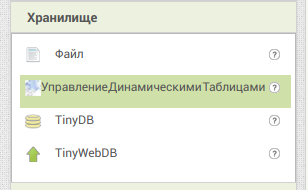
\includegraphics{./lessons/db_google_fusion/01_storage_and_db_types.png}}%
}%
%
\includegraphics{./commons/Flag_of_Republika_Srpska.png}
    \caption{В <<Дизайнере>> в меню <<Палитра>> развёрнута вкладка <<Хранилище>> 
    со списком доступных способов хранения данных: файл и три базы данных}
\label{fig:storage_and_db_types}
\end{marginfigure}

Справа от названия типа хранилища есть значок вопроса (рис.~\ref{fig:storage_and_db_types}). 
Если нажать на значок, то всплыёт окно с подсказкой и рассказом, 
что это за база и как с ней работать.

Вопросы (todo answers and goto links): 
\begin{itemize}
    \item Назовите сайты и программы, которым необходима для работы база данных.
    \item Почему переменная называется <<переменной>> или по-английски ``variable''? 
        Данные в базе являются переменными или константами?
    \item Кто дольше живёт ‒ переменная или константа? (упомянуть рассказ Лема о роботе-дубликате, 
    который симулировал работу, чтобы его не выключили)
    \item Зачем хранить данные в базе данных, если уже есть переменные?
\end{itemize}

\chapter{База данных Google Fusion Tables, она же ДинамиТ}
\label{ch:dynamite}


\newthought{По-английски эта база данных} в App Inventor называется ``FusiontablesControl'', 
в книге Камриани и Роя\cite{KamrianiAndRoy2016} её называют ``Google Fusion Tables''. 
В русском интерфейсе среды App Inventor эта база называется предлинно: 
<<УправлениеДинамическимиТаблицами>>, а мы эту базу данных назовём кратко <<ДинамиТ>>, 
где заглавная буква Т указывает на <<\textbf{Т}аблицы>>.

Программы, работающие с ДинамиТом, должны получить разрешение у сервера Гугл, то есть должны указать логин и пароль. Есть два варианта:
\begin{itemize}
    \item Разработчик приложения получает секретный ключ (API Key) и использует его в программе. 
        В этом случае пользователю программы тоже нужно залогиниться в Google для доступа к ДинамиТу. 

    \item Можно использовать Service Account. Тогда нужно создать 
        файл с логином и паролем (это наш секретный ключик) и получить 
        мейл ``Service Account Email Address'' из Google APIs Console. 
        Затем сообщаем ДинамиТу мейл ``Service Account Email Address'' 
        и загружаем файл с секретным ключиком в своё приложение, 
        и связываем свойство KeyFile с этим файлом. 
        Наконец, в Дизайнере ставим галочку на пункт ``UseServiceAuthentication''. 
        В случае использования Service Account 
        пользователям не нужно заботиться о логине в ДинамиТе, 
        все эти заботы берёт на себя приложение.
\end{itemize}




\section{Приготовление ДинамиТа}


Откройте веб-страницу Google Диска (https://drive.google.com).\marginnote[-0cm]{
    Чтобы получить доступ к Google Диску, достаточно зарегистрироваться на сайте \href{https://www.google.com/}{Google.com}.
}
Нажмите последовательно 
кнопки меню: <<Создать>>, <<Ещё>> и~кнопку <<+ Подключить другие приложения>> 
(рис.~\ref{fig:google_drive_connect_more_apps}). В новом окне будет множество 
приложений, которые можно подключить к~Google Диску. 

\begin{figure}
{%
\setlength{\fboxsep}{0pt}%
\setlength{\fboxrule}{1pt}%
\fcolorbox{gray}{gray}{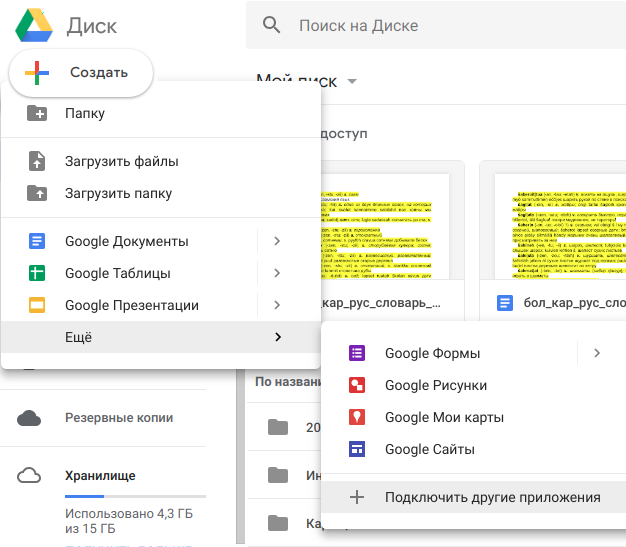
\includegraphics{./lessons/db_google_fusion/020_google_drive_connect_more_apps_with_new-button_ru.png}}%
}%
    \caption[Подключения приложения к Google Диску.][56pt]{Подключения 
            приложения к Google Диску.
    }
  \label{fig:google_drive_connect_more_apps}
\end{figure}

В строке поиска нового окна наберите слово ``Fusion''. Нажмите кнопку поиска. 
Из списка приложений выберите ``Fusion Tables'' и нажмите кнопку <<Подключить>> 
(рис.~\ref{fig:add_fusion_to_drive}).

\begin{figure}
{%
\setlength{\fboxsep}{0pt}%
\setlength{\fboxrule}{1pt}%
\fcolorbox{gray}{gray}{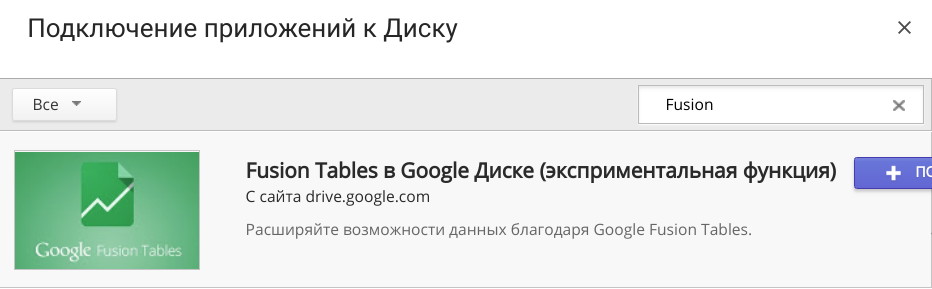
\includegraphics{./lessons/db_google_fusion/030_add_fusion_to_drive_ru.png}}%
}%
    \caption[Выбор приложения в Google Диск.][-0pt]{Выбор приложения 
            ``Fusion Tables'' в Google Диск. У кнопки <<Подключить>> 
            на экране поместились первые полторы буквы.

        { Если даже у Гугля на картинке есть опечатки, то какой может быть 
        спрос с авторов этой книги $\ddot\smile$
        }
    }
  \label{fig:add_fusion_to_drive}
\end{figure}

Теперь, если снова нажать кнопки <<Создать>> и <<Ещё>>, в~списке меню будут 
<<Google Сводные таблицы>> (рис.~\ref{fig:fusion_is_available_at_drive}).
Щёлкнем по кнопке <<Google Сводные таблицы>>, чтобы создать новую таблицу.

\begin{figure}
{%
\setlength{\fboxsep}{0pt}%
\setlength{\fboxrule}{1pt}%
\fcolorbox{gray}{gray}{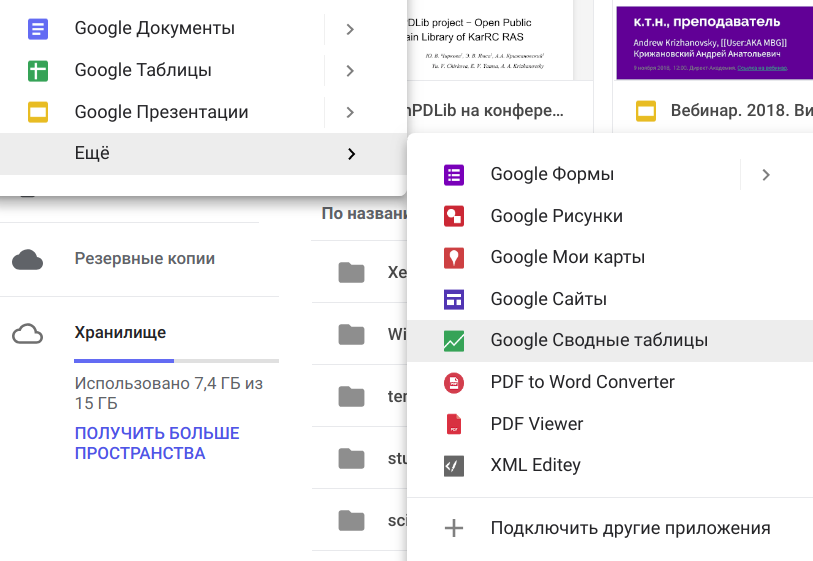
\includegraphics{./lessons/db_google_fusion/040_GoogleFusionTables_avail_ru.png}}%
}%
    \caption[Google Сводные таблицы доступны в Google Диск.][56pt]{Google Сводные таблицы 
            (по-нашему ДинамиТ) доступны в Google Диск.
    }
  \label{fig:fusion_is_available_at_drive}
\end{figure}

Откроется новое окно (рис.~\ref{fig:fusion_create_empty_table}). Выберите пункт 
``Create empty table'' для создания новой пустой таблицы.

\begin{figure}
{
\setlength{\fboxsep}{0pt}%
\setlength{\fboxrule}{1pt}%
\fcolorbox{gray}{gray}{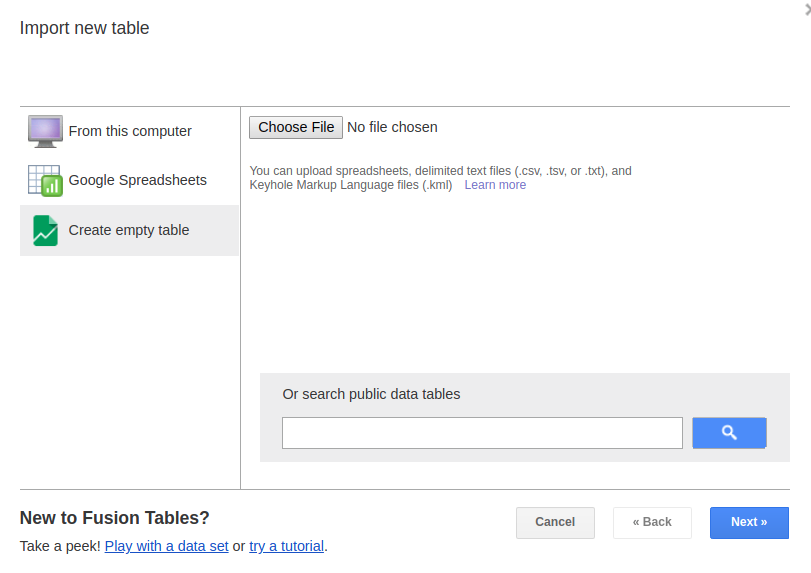
\includegraphics{./lessons/db_google_fusion/050_create_empty_table.png}}%
}
    \caption[Создание новой Google Сводной таблицы.][0pt]{Создание новой 
            Google Сводной таблицы (Fusion Table).

            { 
                Интерфейс Fusion Tables на русский пока не переведён, 
                но для нас это не беда. 
            }

            {
                Обратите внимание, что внизу иллюстрации есть ссылка на учебник 
                по Fusion Tables: \url{https://support.google.com/fusiontables}.
            }
    }
  \label{fig:fusion_create_empty_table}
\end{figure}




\section{Закладка (данных) ДинамиТа}

Ну вот, наконец, мы добрались до табличной формы, 
где можно вводить данные в ДинамиТ или Google Сводные таблицы.

Первым делом дадим таблице название и описание (рис.~\ref{fig:fusion_table_name}). 
Таблицу назовём ``FlagColor Table''. После ввода текста нажмите кнопку ``Save'', 
чтобы сохранения данных.

\begin{marginfigure}[0.0cm]
{
\setlength{\fboxsep}{0pt}%
\setlength{\fboxrule}{1pt}%
\fcolorbox{gray}{gray}{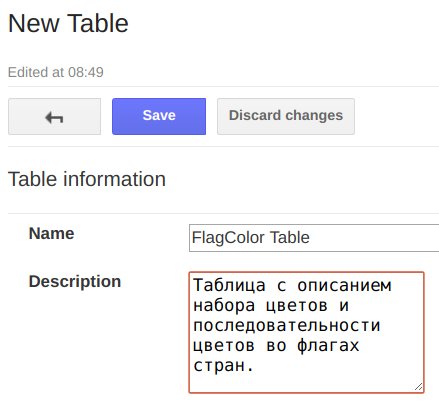
\includegraphics{./lessons/db_google_fusion/060_table_name.png}}
}
    \caption{Переименование новой Google Сводной таблицы (Fusion Table).}
  \label{fig:fusion_table_name}
\end{marginfigure}


\newthought{О пустоте}. Нужна ещё пара штрихов, прежде чем мы сможем использовать эту таблицу в нашем приложении. 
Изначально, при создании таблицы, в неё вставляется одна пустая строка, а нам нужна совершенно пустая таблицу. Как очистить таблицу? 
Для этого выберите пункт меню ``Edit'', затем ``Delete all rows'' (рис.~\ref{fig:fusion_table_delete_all_rows}). 
На вопрос -- уверены ли вы, что нужно всё удалить? -- ответьте утвердительно (рис.~\ref{fig:fusion_table_yes_delete_all_rows}).

\begin{figure}
{
\setlength{\fboxsep}{0pt}%
\setlength{\fboxrule}{1pt}%
\fcolorbox{gray}{gray}{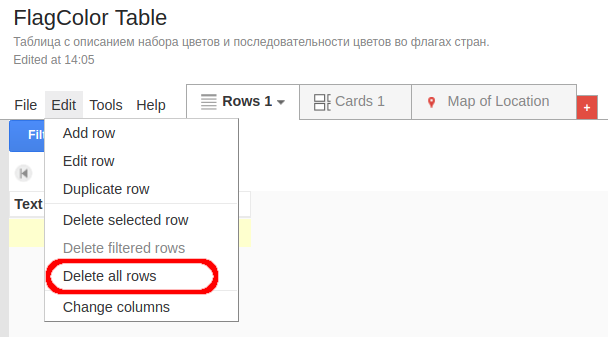
\includegraphics{./lessons/db_google_fusion/070_Edit_delete_all_rows_to_clear_table.png}}
}
    \caption[Очистка Сводной таблицы.][0pt]{Удаление всех строк для очистки таблицы.
            {
                Пункты меню ``Edit'', затем ``Delete all rows''.
            }
    }
  \label{fig:fusion_table_delete_all_rows}
\end{figure}


\begin{marginfigure}[0.0cm]
{%
\setlength{\fboxsep}{0pt}%
\setlength{\fboxrule}{1pt}%
\fcolorbox{gray}{gray}{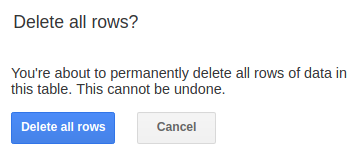
\includegraphics{./lessons/db_google_fusion/080_yes_delete_all_rows.png}}%
}%
%
\includegraphics{./commons/Flag_of_Republika_Srpska.png}
    \caption{Подтверждение удаления всех строк таблицы.}
\label{fig:fusion_table_yes_delete_all_rows}
\end{marginfigure}


\newthought{К вводу данных} можно уже и приступить. 
Определим для себя, какие столбцы нам нужны для использования таблицы 
в главе \ref{ch:draughts-moves} <<Превращение флагов>> (с.~\pageref{ch:draughts-moves}). 
Нужны четыре столбца:

\begin{description}
    \item[country] -- текстовое поле для названия страны (например, ``Russia'', ``Gabon''),
    \item[row] -- числовое поле для указания номера полоски цвета, считаем сверху вниз, отсчёт начинаем с единицы,
    \item[hex-triple?] -- числовое? поле для указания RGB-цвета,
    \item[color-name] -- текстовое поле для названия цвета, служит human-readable комментарием к RGB-коду!
\end{description}





\chapter{Превращение флагов}
\label{ch:draughts-moves}

\begin{marginfigure}[-2em]
{%
\setlength{\fboxsep}{0pt}%
\setlength{\fboxrule}{1pt}%
\fcolorbox{gray}{gray}{
\includegraphics{./commons/Flag_of_Republika_Srpska.png}}%
}%
%
\includegraphics{./commons/Flag_of_Republika_Srpska.png}
%\fcolorbox{white}{gray}{
\includegraphics{./commons/Flag_of_Republika_Srpska.png}}

\caption{Флаг Сербии. Какие ещё два флага можно получить, слегка меняя оттенки 
    и сдвигая горизонтальные полоски вверх или вниз? 
    См. ответ~\ref{answer:Tricolor-flags} на с.~\pageref{answer:Tricolor-flags}.}
\label{fig:Srpska}
\end{marginfigure}

\newthought{В нашей задаче} будет дана стопка горизонтальных полосок разных цветов, 
из которых можно составить флаги государств. Сначала в игре показывают такие флаги и сообщают названия государств.
Игроку нужно расположить горизонтальные полоски так, чтобы они составили какой-либо известный флаг. 

Сузим задачу, ограничимся только трёхцветными флагами, как у России 
или Сербии (рис.~\ref{fig:Srpska}).
А по цветовой гамме выберем только флаги с белыми, синими или красными цветами.

\newthought{Сколько} таких флагов? И у каких государств? Ответы на эти вопросы 
можно найти с помощью Викиданных %\marginnote{
% }. 
На Викиданных представлены \href{http://bit.ly/2OgIdWo}{328 государственных флага}\footnote[][-3cm]{
    SPARQL-запрос к Викиданным для получения списка государственных флагов: \url{http://bit.ly/2OgIdWo}
}, 
причём с тремя горизонтальными полосками по версии Викиданных 
существует \href{http://bit.ly/2Q96ET1}{101 флаг}\footnote[][-2.8cm]{
    Список горизонтальных триколоров по Викиданным
    \url{http://bit.ly/2Q96ET1}
}. 
Горизонтальных триколоров с красным, белым и синим цветом 
имеют всего \href{http://bit.ly/2xDTXsI}{19 государств}\footnote[][-2.0cm]{
    Только синие, белые и/или красные цвета у триколоров 
    \url{http://bit.ly/2xDTXsI}
    \bigskip 
}.

\marginnote[-0.5cm]{
    О языке SPARQL и объектах Викиданных читайте в курсе Викиверситета ``Программирование Викиданных'' 
    \href{https://ru.wikiversity.org/wiki/\%D0\%9F\%D1\%80\%D0\%BE\%D0\%B3\%D1\%80\%D0\%B0\%D0\%BC\%D0\%BC\%D0\%B8\%D1\%80\%D0\%BE\%D0\%B2\%D0\%B0\%D0\%BD\%D0\%B8\%D0\%B5_\%D0\%92\%D0\%B8\%D0\%BA\%D0\%B8\%D0\%B4\%D0\%B0\%D0\%BD\%D0\%BD\%D1\%8B\%D1\%85}{https://ru.wikiversity.org}.
}

\begin{mdfstyle}[nobreak=true,frametitle=На каком языке компьютеры читают Википедию?]
\sloppy 
    \index{Викиданные}Викиданные -- это компьютерная система, включающая базу данных, интерфейс для редактирования и язык запросов SPARQL для поиска в базе. Как и Википедию, Викиданные может редактировать каждый. Программисты любят Викиданные, потому что это та же Википедия, но в машиночитаемом виде, то есть язык Викиданных понимают и роботы, и компьютерные программы.
% \marginnote{Hello}
\end{mdfstyle}

\begin{marginfigure}[-4cm]
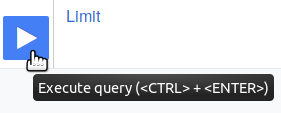
\includegraphics{./wikidata/play_blue_button_wikidata.png}
%\fcolorbox{white}{gray}{
\includegraphics{./commons/Flag_of_Republika_Srpska.png}}

    \caption[Кнопка Play на странице выполнения SPARQL-запросов к Викиданным]{Кнопка 
    Play на странице ``Wikidata Query'' для запуска SPARQl-скриптов.
    Вместо клика по кнопке можно нажать комбинацию клавиш <Ctrl>+<Enter>.}
  \label{fig:blue:button}
\end{marginfigure}

\begin{marginfigure}[-0cm]
  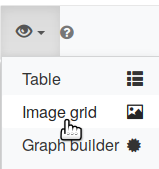
\includegraphics[width=0.5\columnwidth]{./wikidata/image_grid_select.png}
%  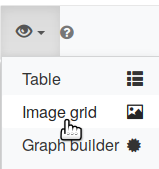
\includegraphics{./wikidata/image_grid_select.png}
  \caption[Выбор представления результатов SPARQL-запроса в виде мозаики 
    иллюстраций.]{Выбор представления результатов SPARQL-запроса 
    в виде мозаики иллюстраций. Нажмите на значок глАза, затем выберите 
    пункт ``Image grid'' в выпадающем меню.
}
  \label{fig:wd:grid:select}
\end{marginfigure}


\newthought{Эти короткие ссылки}, например, \url{http://bit.ly/2OgIdWo}, 
приведут вас на страницу ``Wikidata Query'', 
то есть на страницу запросов к базе Викиданных на языке SPARQL. 
Чтобы запустить запрос, нажмите на кнопку Play (рис.~\ref{fig:blue:button}). 
Для превращения скучного списка названий флагов в мозаику флагов, 
щёлкните по значку глАза, затем выберите пункт выпадающего меню 
``Image grid'' (рис.~\ref{fig:wd:grid:select}).% \sidenote[][-3.0cm]{This sidenote is 1 centimeter higher than it normally would be and uses its original sidenote number.}





\begin{mdframed}[nobreak=true]
\sloppy % Text doesn't wrap correctly inside an mdframed frame (in tufte-book), see https://tex.stackexchange.com/a/153877/99685
    \index{Короткая ссылка}Короткие ссылки создаются специальными сайтами, которые берут длиннющую 
    гиперссылку и превращают её в коротенький набор букв и цифр. Это удобно, 
    если вы хотите оставить место в сообщении для своего текста и 
    не тратить драгоценные знакоместа на кашу из символов в URL.  
    Таких сервисов по сокращению URL много, bit.ly -- это один из них. 
    А почему сервис bitly называется bitly? Потому что ссылки становятся "a little BIT smaller", то есть "чуть-чуть покороче". 
    И потому что ``бит'' (англ. bit) -- это крошечное количество данных. 
    % Source: Why is it called Bitly? Annelise Schoups, 2016. URL: https://www.rewindandcapture.com/why-is-bitly-called-bitly/
\end{mdframed}

\begin{marginfigure}[-4cm]
{%
\setlength{\fboxsep}{0pt}%
\setlength{\fboxrule}{1pt}%
%\fcolorbox{gray}{gray}{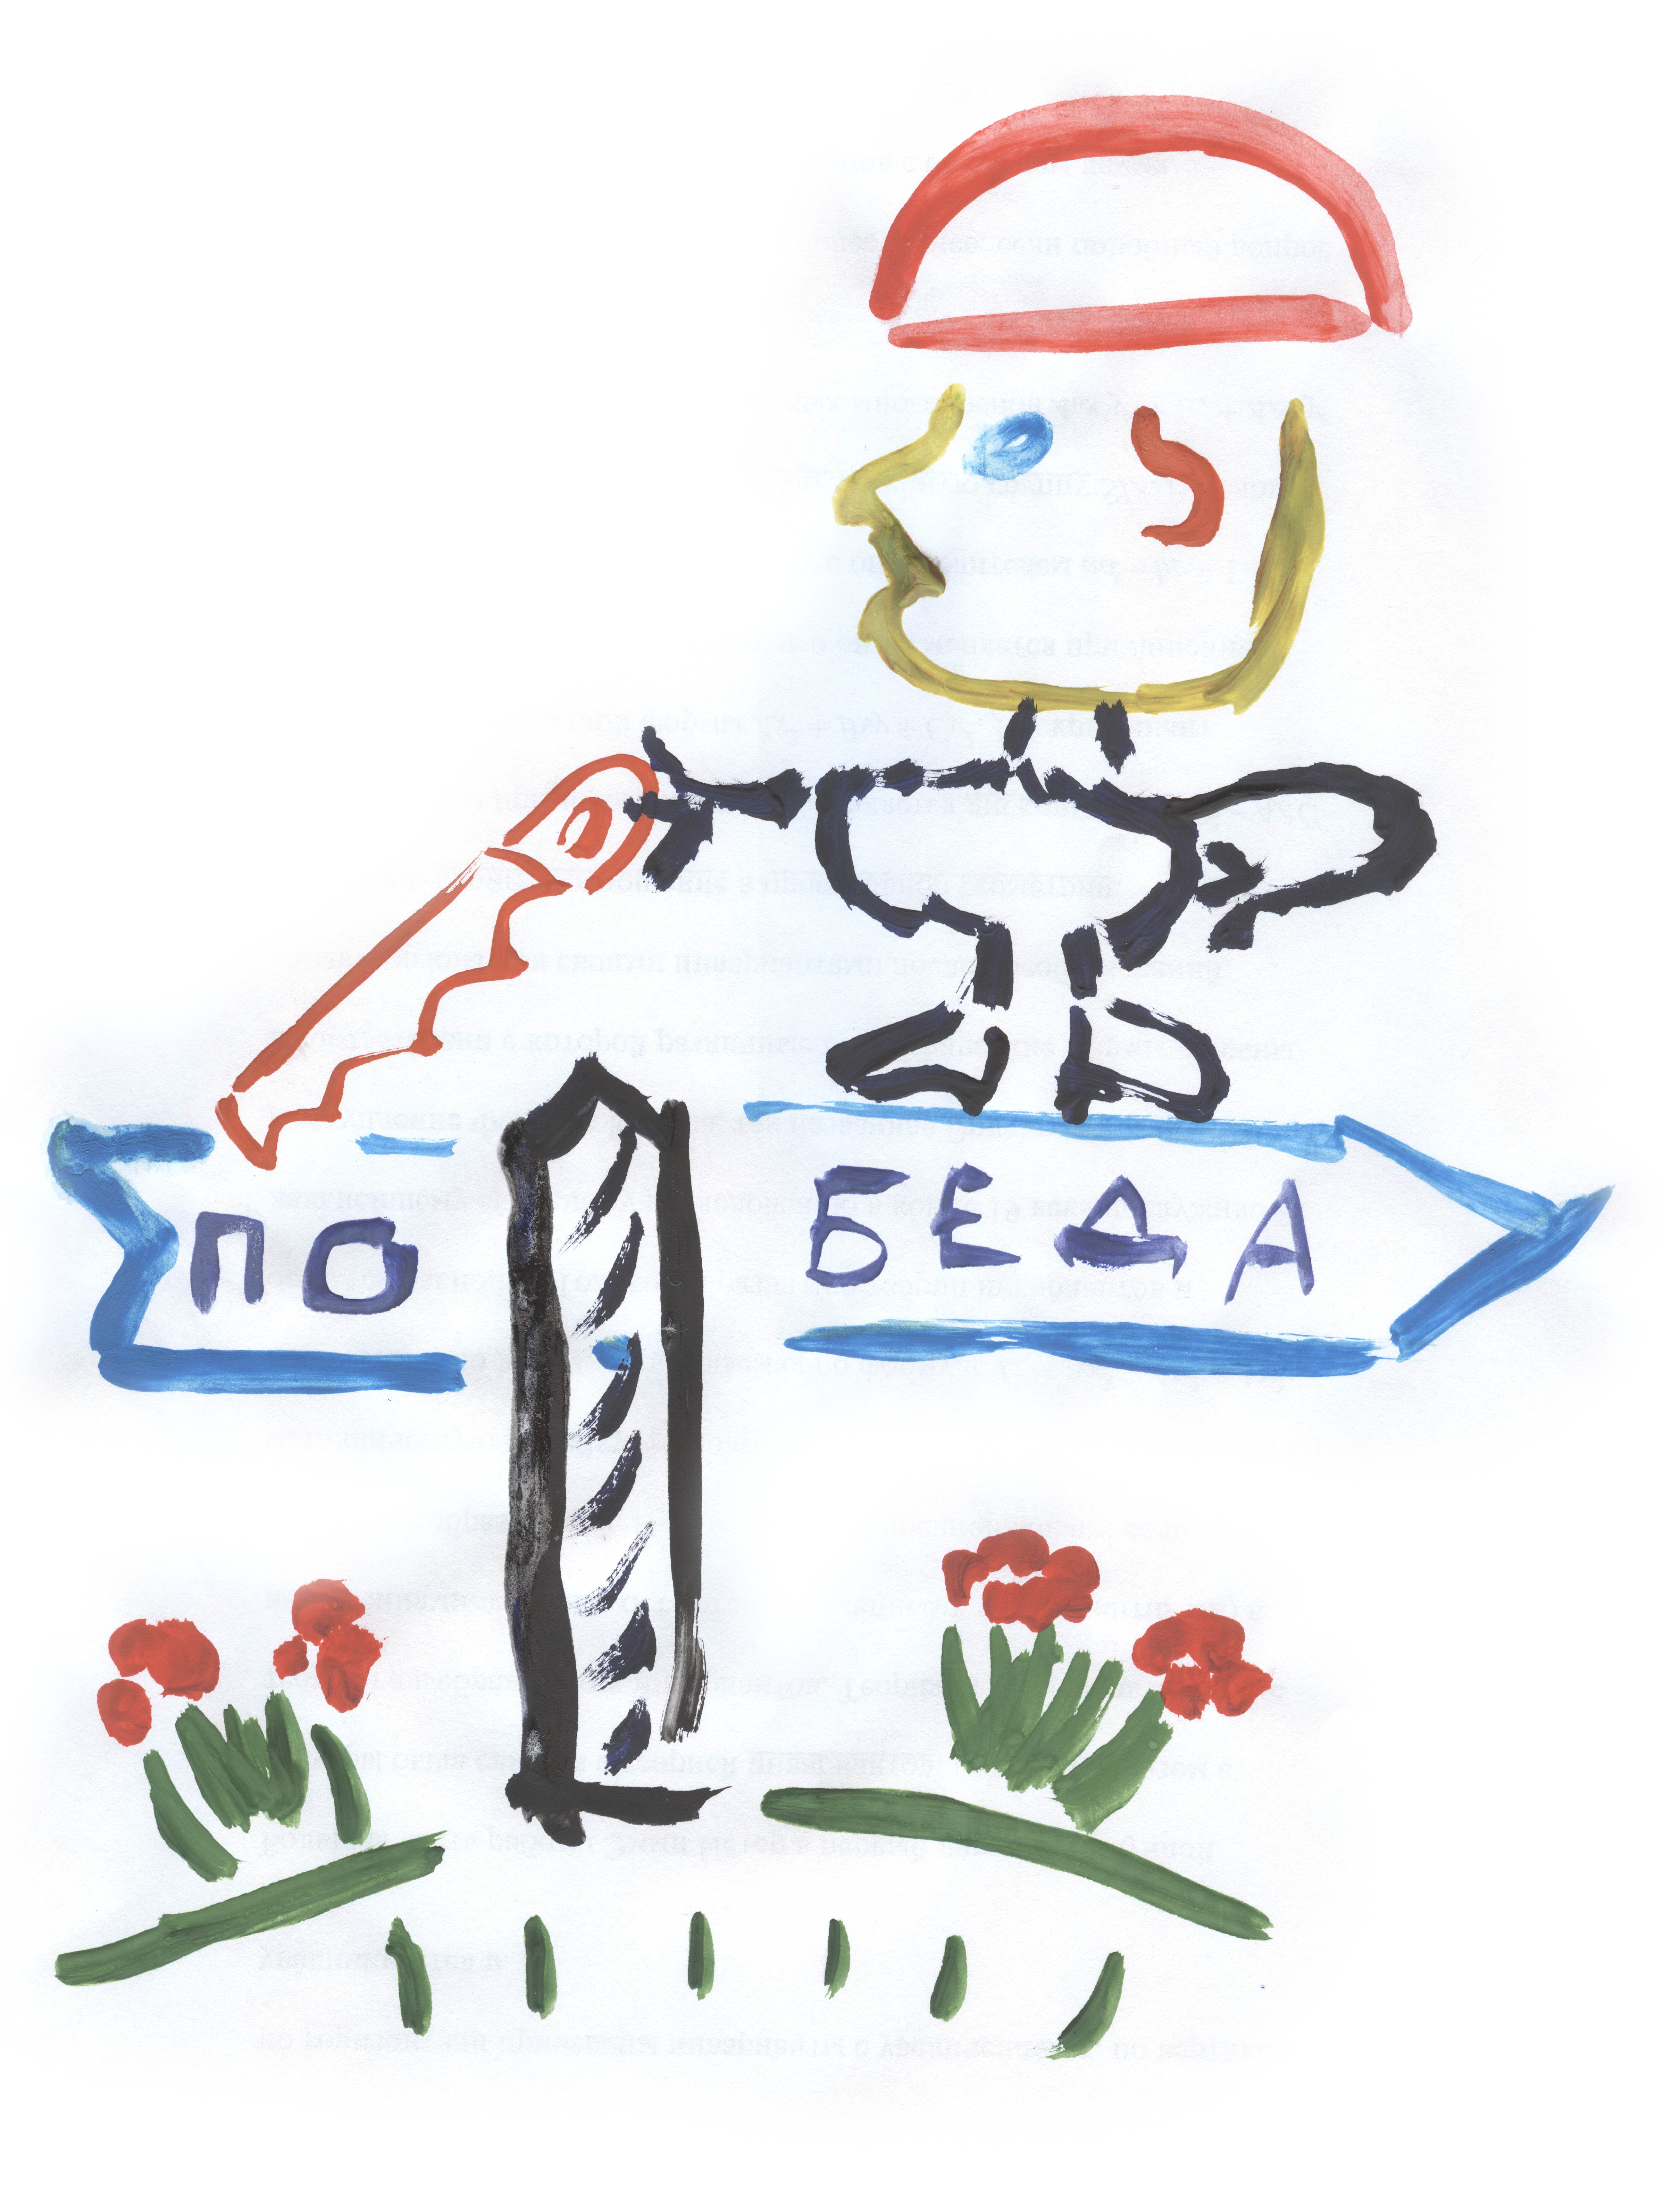
\includegraphics{./graphics/sketch/short_link_knauff_pobeda_v3.jpg}}%
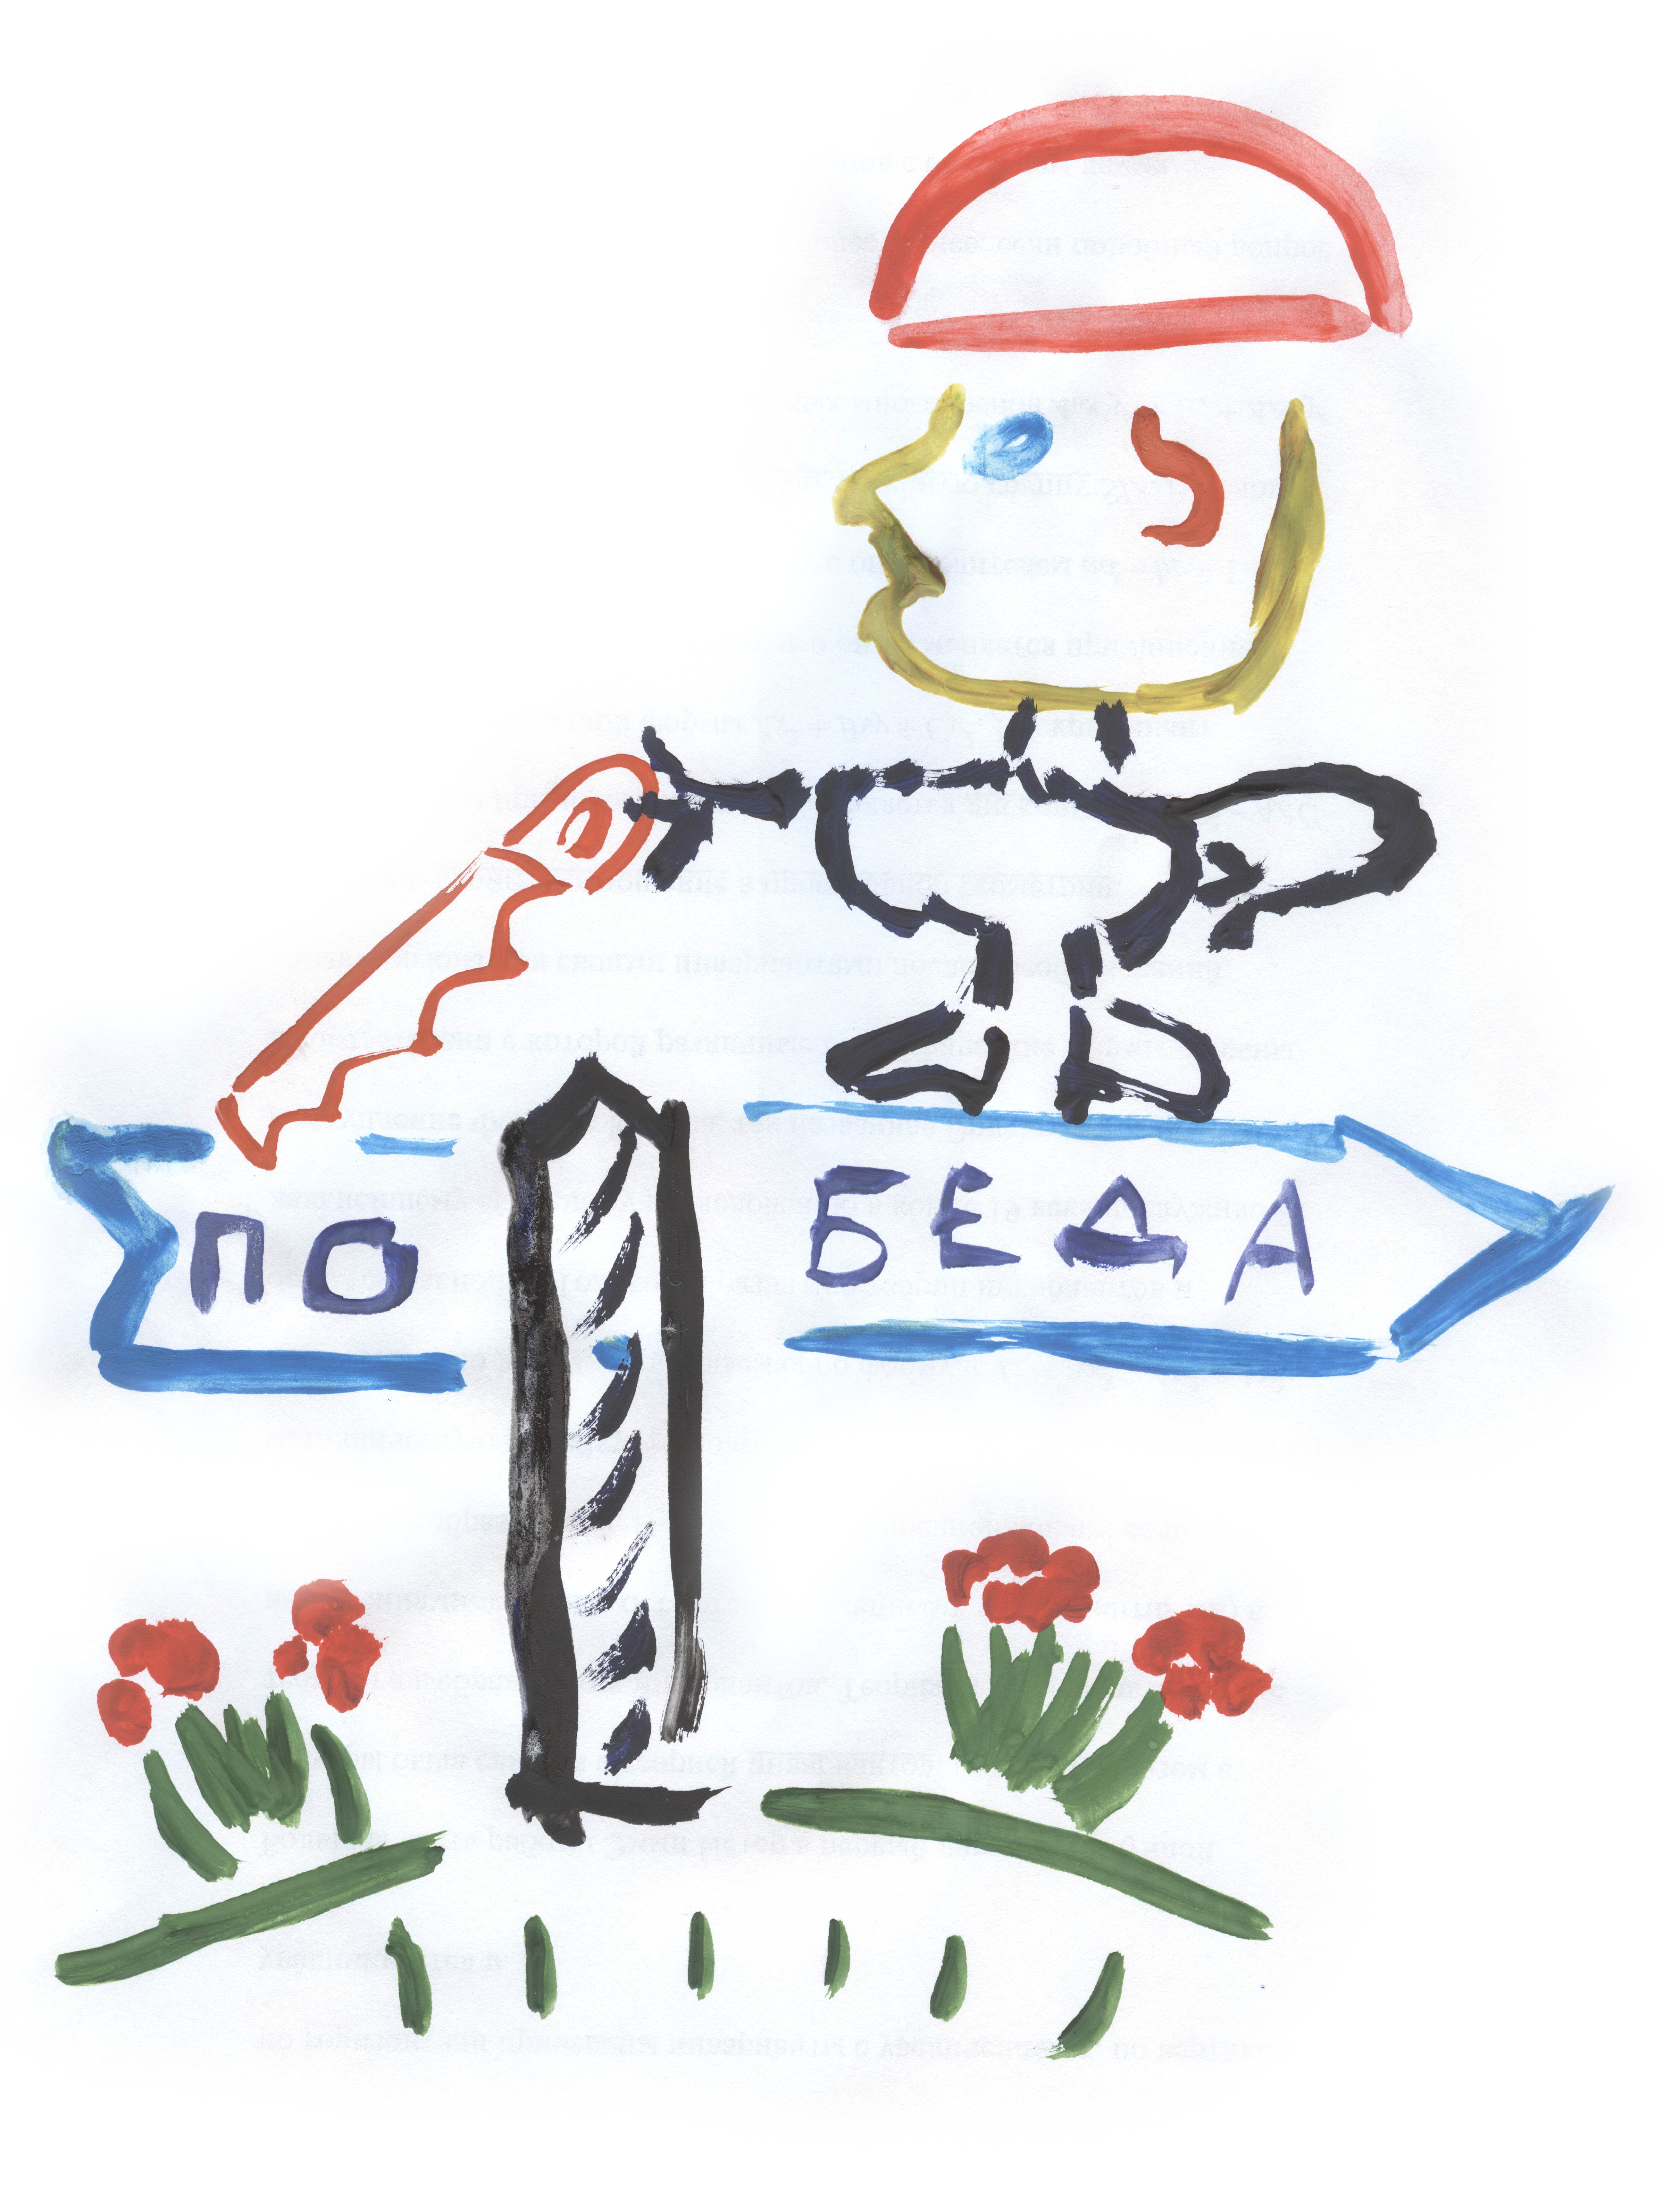
\includegraphics{./graphics/sketch/short_link_knauff_pobeda_v3.jpg}
}%
%
\includegraphics{./commons/Flag_of_Republika_Srpska.png}
%\fcolorbox{white}{gray}{
\includegraphics{./commons/Flag_of_Republika_Srpska.png}}

\caption{Есть разные подходы и алгоритмы для укорачивания ссылок и имён. В~каком 
    мультфильме название корабля в начале плавания стало короче задуманного и почему?
    См. ответ~\ref{answer:Pobeda-beda} на с.~\pageref{answer:Pobeda-beda}.}
\label{fig:Pobeda-beda}
\end{marginfigure}

Задача: сколько ссылок можно закодировать, 
        если ссылка содержит ровно 7 буквенно-цифровых символов,
        каждый символ может быть буквой английского алфавита 
        или цифрой от 0 до 9? Ответ на странице ... todo.

Temp indexkey example: А вот и \index{Интерфейс пользователя!ListView / Выбор из списка}...

\newthought{В нашей программе цвета полосок} -- это то, чем мы будем управлять, 
чтобы построить нужный флаг. 

Создадим глобальную переменную \var{colors} для хранения наших цветов 
(может, переменную стоило назвать <<ваза>>? $\ddot\smile$). 
Создадим список\footnote[][-2cm]{\emph{Список} (list) -- это структура для хранения данных. 
Например, названия предметов \{\emph{математика, история, русский}\} -- это тоже список.
} 
из четырёх цветов и присвоим список глобальной\footnote[][-0cm]{\index{Переменная!глобальная}
    \emph{Глобальная переменная} по-английски 
    называется ``global variable''. К ней можно обратиться из любого места программы. 
    }\marginnote[0.2cm]{
    Чем хороши глобальные переменные и какие у них недостатки
    по сравнению с локальными переменными? 
    См. ответ~\ref{answer:global-vars-pros-cons} на с.~\pageref{answer:global-vars-pros-cons}.
}
переменной \var{colors}. См. верхнюю строчку на рис.~\ref{fig:block:proc:swap:colors}.

\begin{figure}
  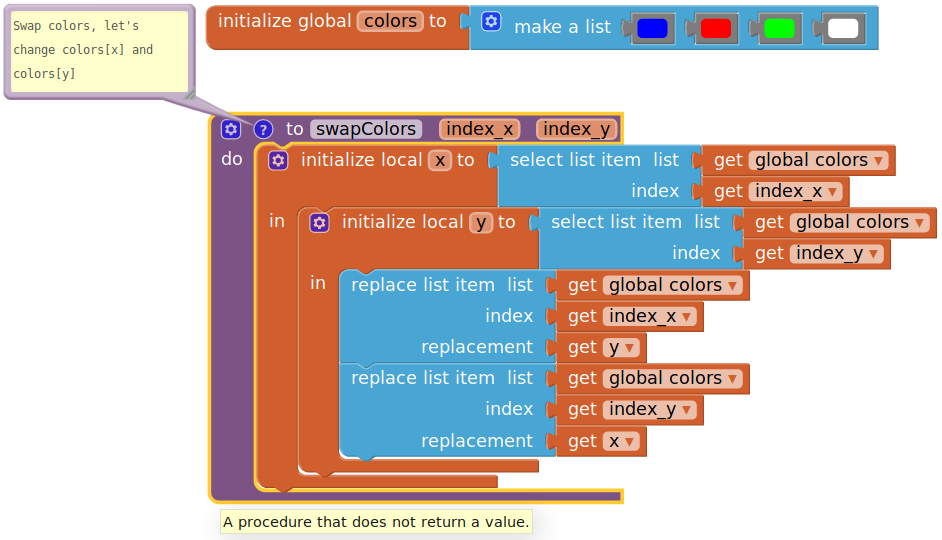
\includegraphics{./graphics/programs/change_flags/proc_swap_colors_2018.png}
    \caption[Процедура \var{swapColors}.][56pt]{Процедура \var{swapColors}.
    Аргументы процедуры -- номер первого цвета (\var{index\_x}) 
    и номер второго (\var{index\_y}). 
    Например, вызов процедуры \var{swapColors(1,3)} поменяет местами первый и 
    третий цвета (синий и зелёный) в списке \var{colors}. 
    
    {\tiny Написать рядом то же, что и на рисунке, но в виде псевдокода, 
    см. https://tex.stackexchange.com/a/381105/99685
    }
    
    }
  \label{fig:block:proc:swap:colors}
\end{figure}

Используем объект "canvas" при создании интерфейса программы, чтобы нарисовать 
цветные полоски ... TODO

Следующий код позволит игроку щёлкать по полоскам 
и две ближайшие полоски будут меняться местами. 
Для этого нам пригодится процедура "SwapColors" (todo figure ref). 

\begin{figure}
  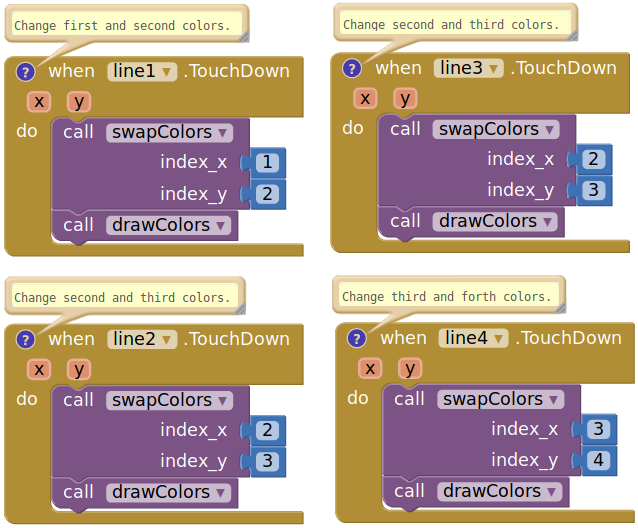
\includegraphics{./graphics/programs/change_flags/click_and_swap_colors_2018.png}
    \caption[Caption short.][6pt]{Caption long.
    }
  \label{fig:block:click:swap:colors}
\end{figure}

TODO Почему комментарии и названия переменных на английском языке?

\chapter{Угадыватель чисел}
\label{ch:guessnumbers}

В этой главе мы познакомим вас с программой <<Угадыватель чисел>>\cite{PanfilovaApp}, идея которой взята из книги Л. Ф. Магницкого «Арифметика»\cite{Galanin}. 
Опишем задачу и расскажем, как запрограммировать решение. Поработаем с экранами приложения, создадим процедуры и покажем как разрешить ввод только числовых значений в программе.


\section{Описание задачи}

Суть предлагаемой нами задачи описана в книге Л. Ф. Магницкого, «Арифметика», в главе: «Об утешных некиих действиях, через арифметику употребляемыx»\cite{Galanin}.

Пронумеруем дни недели от одного (понедельник) до семи (воскресенье). 
Предложим игроку загадать число, равное номеру любого дня недели. Далее попросим загадавшего выполнить следующие действия:
\begin{enumerate}
\item Умножить номер загаданного дня недели на два\footnote[][-0cm]{Шаг 1.}\marginnote[0.2cm]{Пусть $ a $ — искомое число (день недели), $ a \in [1;7] $. В результате выполнения шага 1 получаем $2\cdot a $}. 
\item К полученному произведению прибавить пять\footnote[][-0cm]{Шаг 2.}\marginnote[0.2cm]{$2\cdot a + 5$}.
\item Затем полученную сумму умножить на пять\footnote[][-0cm]{Шаг 3.}\marginnote[0.2cm]{$5\cdot(2 \cdot a  + 5) = 10 a + 25$}.
\item Полученное число умножить на десять\footnote[][-0cm]{Шаг 4.}\marginnote[0.2cm]{$(10a + 25)\cdot 10 = 100  a + 250$}.
\item Назвать результат вычислений.
\end{enumerate}

Чтобы перейти от полученного числа к загаданному, необходимо вычесть из него двести пятьдесят и поделить полученное число на сто\footnote[][-0cm]{Определяем число, загаданное игроком: $\frac{100  a + 250 - 250}{100} =  a $}. 

Таким образом, с помощью этих арифметических преобразований мы определили, какое число загадал игрок, то есть нашли~$a$.
\begin{mdfstyle}[nobreak=true,frametitle=Вопрос о числовых множествах]
  \sloppy 
  При постановке задачи мы указали, что а это номер дня недели, то есть натуральное число, $ a \in \mathbb{N} $ . Будет ли работать наш алгоритм угадывания для чисел из множеств $\mathbb{Z}, \mathbb{Q}, \mathbb{R} $? И что это за множества?  
  Ответ на странице \pageref{answer:guess_numbers_task}.
  \label{question:text}
\end{mdfstyle}

\section{Реализация приложения}
\label{styles}
В программе «Угадыватель чисел» (The Numbers Guessing Game)\cite{PanfilovaApp} загаданный игроком номер дня недели — это то, что мы будем искать.
Создадим глобальную переменную  \textit{SecretNumber} для хранения искомого числа, загаданного игроком. Присвоим этой переменной значение, равное нулю. 
Так как ноль не входит в интервал от одного до семи, то переменная \textit{SecretNumber} в данный момент не равна загаданному числу $ a $\footnote[][-0cm]{\mbox{$ \left.\begin{array}{ccc}
  SecretNumber = 0 \\
  a \in [1;7] \\
\end{array}
\right\}\Rightarrow SecretNumber \neq a $}}. Это хороший стиль программирования, который позволяет проинициализировать переменную так, чтобы явно указать, что результат ещё не получен. Также
отметим, что в этом приложении объекты именуются в стиле PascalCase\cite{Chase2018}\marginnote[0.2cm]{Именовать объекты можно также произвольно, но рекомендуется использовать один из общепринятых стилей.
  Существуют следующие стили написания составных слов: CamelCase, SnakeCase, KebabCase, PascalCase и другие.
  Подробнее о них можно узнать в статье Чейза Адамса <<Стили написания составных слов в программировании>>}.

\subsection{Определение числа, загаданного игроком}
Чтобы в поле \textit{NumberText} пользователь мог вводить только числовые значения, необходимо поставить галочку у свойства \textit{NumbersOnly} этого поля.

Рассмотрим блок обработки нажатия (рис.~\ref{fig:block:button:click}) на кнопку «Узнать ответ» (Button1).
Когда игрок нажимает на эту кнопку, последовательно выполняются следующие действия:
\begin{figure}
  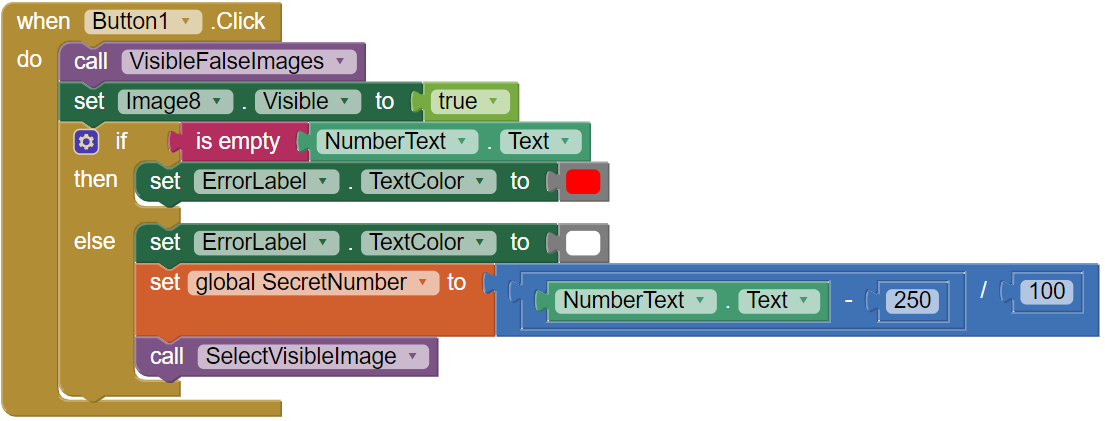
\includegraphics{./graphics/programs/guess_numbers/block_Button1Click_AppInventor_2018.png}
    \caption[Блок обработки нажатия на кнопку Button1.][12pt]{Блок обработки нажатия на кнопку Button1 и сокрытия всех изображений цифр, вывод результата или сообщения об ошибке.}
  \label{fig:block:button:click}
\end{figure}
\begin{enumerate}
  \item Вызываетcя процедура \textbf{VisibleFalseImages} (рис.~\ref{fig:block:visible:false:images}), которая устанавливает свойство Visible у всех изображений с цифрами в false. Таким образом, пока не будет определено число, загаданное пользователем, изображения с цифрами не будут отображаться.
  \begin{marginfigure}[-2em]
    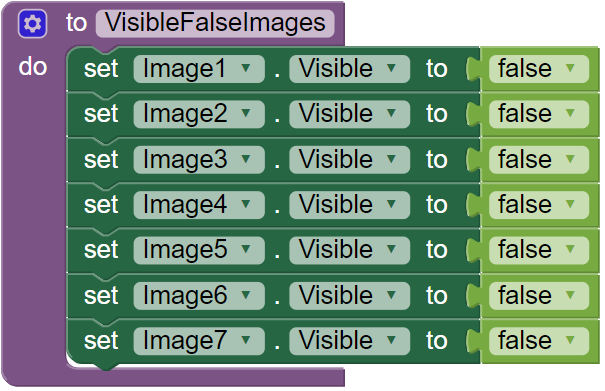
\includegraphics{./graphics/programs/guess_numbers/procedure_visibleFalseImages_AppInventor_2018.png}
      \caption[Процедура VisibleFalseImages.]{Процедура VisibleFalseImages устанавливает свойство Visible у всех изображений с цифрами в false.}
    \label{fig:block:visible:false:images}
  \end{marginfigure}

  \item Устанавливается свойство \textit{Visible} в значение true у изображения со знаком вопроса (Image8).
  \item Если значение поля для ввода загаданного числа (\textit{NumberText}) пусто, то приложение сигнализирует пользователю об ошибке следующим образом. Устанавливаем красный цвет шрифта, чтобы стало видно сообщение «Пожалуйста, введите полученное число» у поля \textit{ErrorLabel} (рис.~\ref{fig:display:error}).
  \begin{marginfigure}[2em]
    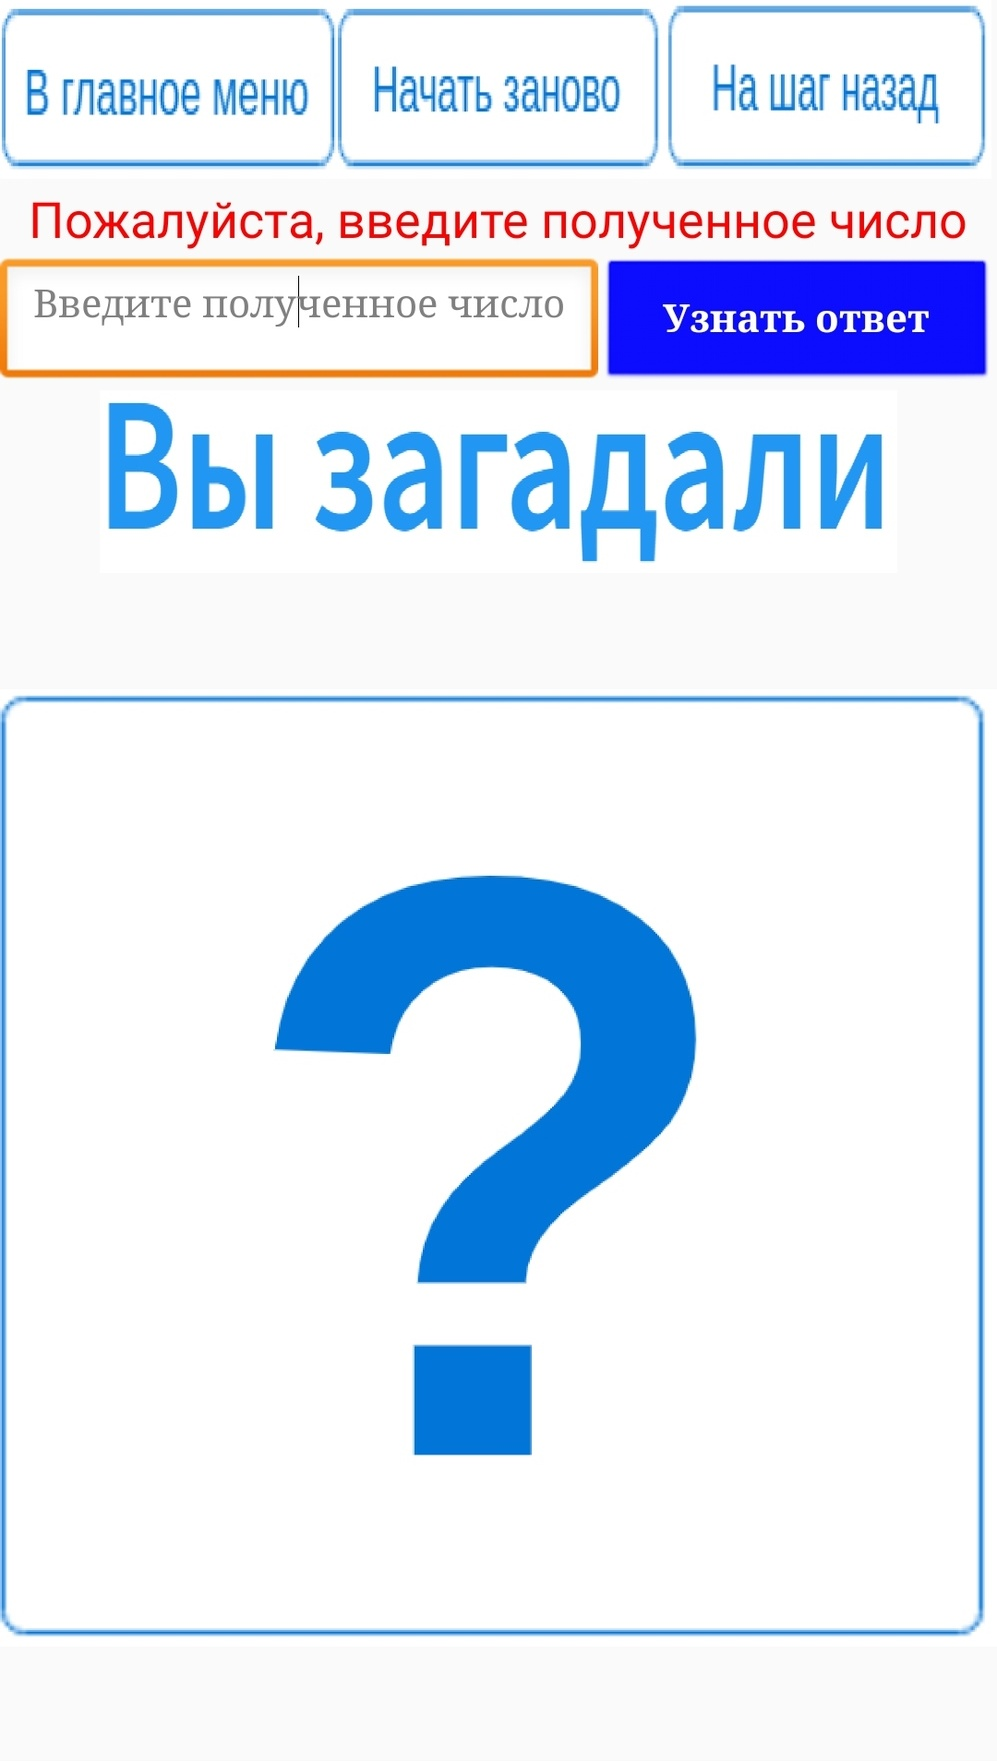
\includegraphics{./graphics/programs/guess_numbers/finalScreen_Error2_TheGuessingNumbersGame_AppInventor.jpg}
      \caption[Сообщение об ошибке на экране FinalScreen.]{Сообщение об ошибке на экране FinalScreen.}
    \label{fig:display:error}
  \end{marginfigure}
  В случае, когда что-либо введено в поле \textit{NumberText}, последовательно выполняются следующие шаги:
  \begin{itemize}
    \item Устанавливается белый цвет шрифта у поля \textit{ErrorLabel}, чтобы скрыть сообщение об ошибке.
    \item Производится подсчёт значения переменной \textit{SecretNumber}.
    \item Вызывается процедура \textbf{SelectVisibleImage}, которая будет рассмотрена далее.
  \end{itemize}
\end{enumerate}
Возникает вопрос: почему для того, чтобы отображать сообщение об ошибке мы меняем цвет текста у поля \textit{ErrorLabel}, а не управляем значением свойства \textit{Visible}? 
Дело в том, что при использовании свойства \textit{Visible}, любое изменение его значения вызывает перерисовку экрана, а элементы интерфейса будут менять свои позиции, то есть <<скакать>> по экрану.
В нашем приложении, если цвет поля белый, то компонент \textit{ErrorLabel} сливается с фоном экрана, сообщения об ошибке не видно.
\section{Процедура SelectVisibleImage}

\begin{figure}
  \includegraphics{./graphics/programs/guess_numbers/procedure_selectVisibleImage_AppInventor_2018.png}
    \caption[Процедура SelectVisibleImage.]{Процедура SelectVisibleImage управляет отображением изображений с цифрами. Пунктирной линией отреза сокращено число однотипных блоков управления, выполняющих действия по установке значения свойства Visible в true у изображения с числом, которое соответствует значению переменной \textit{SecretNumber}. На рисунке такие блоки указаны для чисел один и семь.}
  \label{fig:block:click:select:visible:image}
\end{figure}

Процедура \textbf{SelectVisibleImage} (рис.~\ref{fig:block:click:select:visible:image}) читает значение глобальной переменной \textit{SecretNumber} и отображает рисунок с соответствующей цифрой.
В случае, если число не было определено, показывается изображение с вопросительным знаком (\textit{Image8}).

Например, пусть игрок загадал число три. На основании введённого пользователем числа в поле \textit{NumberText} на экране \textit{FinalScreen}
(пусть в этом примере введено число 550)\footnote[][0.5cm]{ Пусть $ x $ — число, которое должен ввести пользователь, $ a $ — загаданный игроком номер дня недели, $ a \in [1;7] $, $ ] a = 3 $. 

Чтобы найти $ x $ выполним следующие преобразования:

$ x = 100 \cdot a + 250  = 100 \cdot 3 + 250  = 550 $}\marginnote[0.2cm]{} приложение подсчитает и присвоит переменной \textit{SecretNumber} новое значение, равное трём.
Процедура \textit{SelectVisibleImage} в соответствии со значением переменной \textit{SecretNumber} делает видимым изображение с соответствующей загаданному числу цифрой. 
В нашем примере это изображение числа три (\textit{Image3}). Если переменная \textit{SecretNumber} содержит значение, не входящее в интервал от одного до семи, то будет показано изображение со знаком вопроса (\textit{Image8}), а текст надписи \textit{ErrorСalculating} станет видимым (<<Допущена ошибка в расчетах. Попробуйте снова>>, рис.~\ref{fig:block:final:screen:error:label}).
\begin{marginfigure}[-2em]
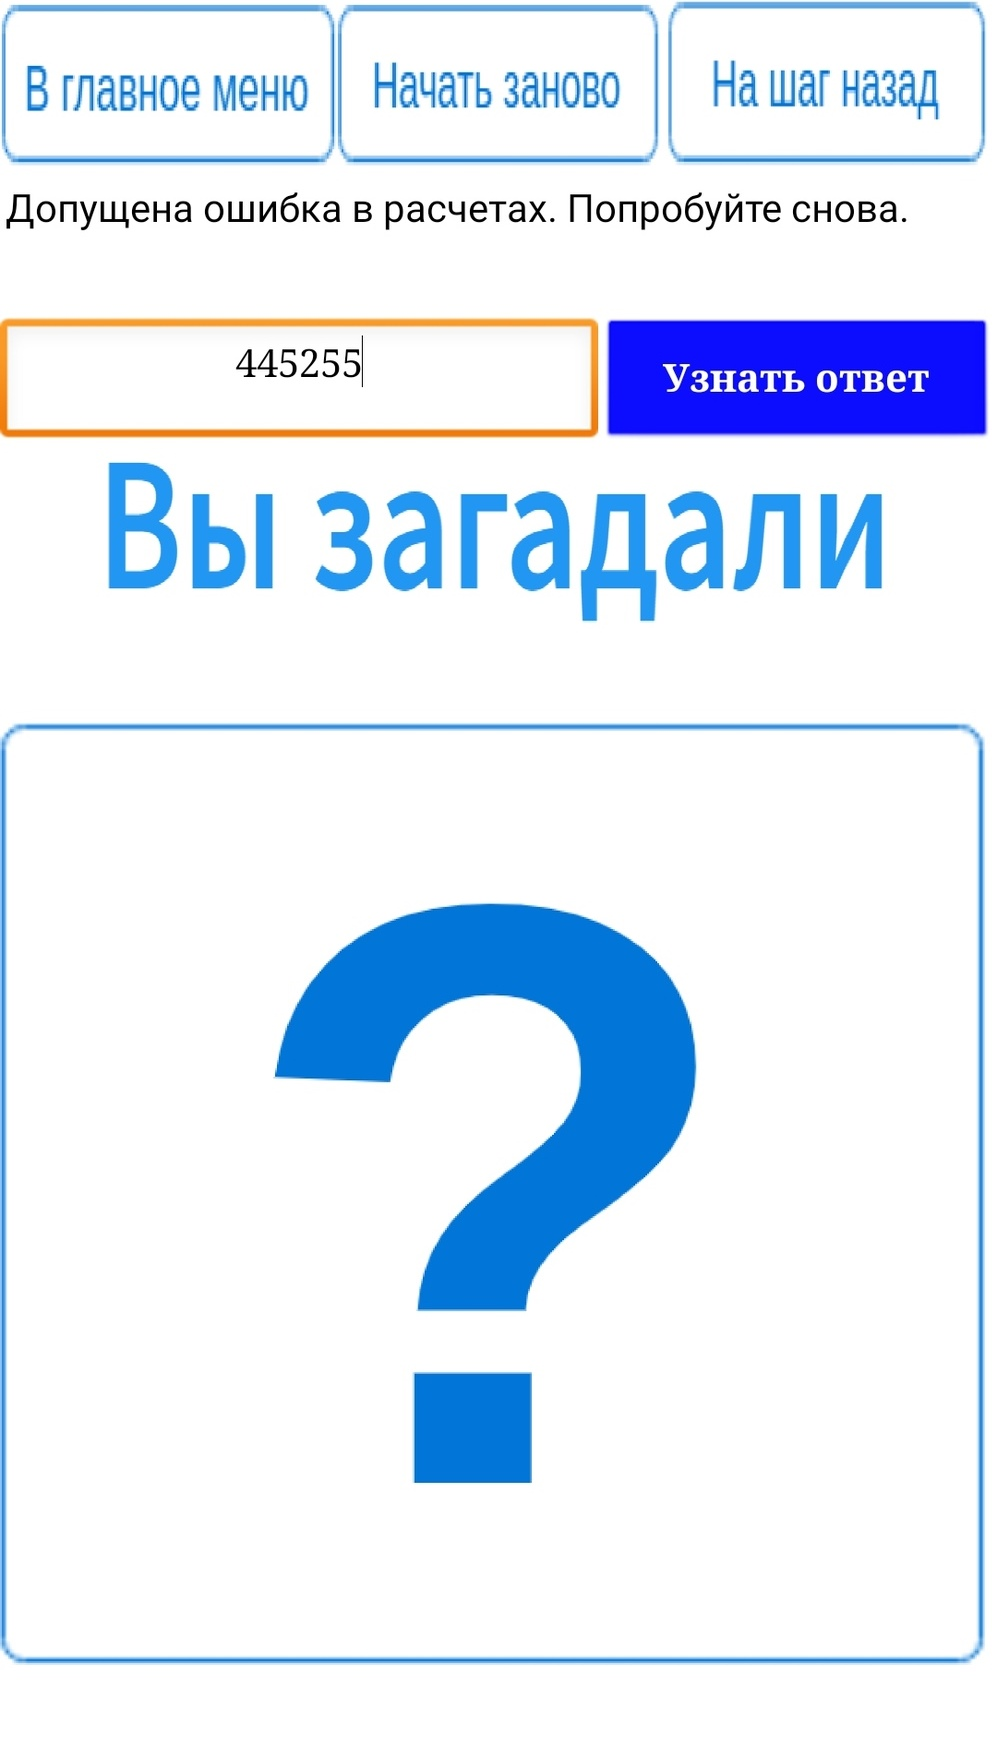
\includegraphics{./graphics/programs/guess_numbers/finalScreen_Error_TheGuessingNumbersGame_AppInventor.jpg}
\caption[Сообщение об ошибке в расчётах на экране FinalScreen.]{Сообщение об ошибке в расчётах на экране FinalScreen.}
  \label{fig:block:final:screen:error:label}
\end{marginfigure}
Важно отметить, что перед выполнением орпераций сравнения переменной \textit{SecretNumber} с введенным пользователем числом, выполняется установка свойства \textit{Visible} в \textit{false} у элементов \textit{Image8} и \textit{ErrorСalculating} (рис.~\ref{fig:block:click:select:visible:image}).
Тем самым мы отмечаем отсутствие ошибок в вычислениях и заранее убираем с экрана знак вопроса, предполагая, что на его месте будет изображение с определённой цифрой. Если же переменная \textit{SecretNumber} не входит в интервал от одного до семи, то у элементов \textit{Image8} и \textit{ErrorСalculating} устанавливается значение свойства \textit{Visible} в \textit{true}, 
так приложение сообщает пользователю о его ошибке в вычислениях.

\subsection{Работа с экранами}
При проектировании приложения были учтены рекомендации из официальной документации App Inventor\cite{MitManyScreens} по ограничению количества экранов во избежание проблем с переполнением памяти.
Поэтому в игре используется восемь экранов (рекомендуемое количество — меньше 10):
\begin{enumerate}
\item \textbf{Screen1} — главный экран приложения, меню игры.
\item \textbf{About} — экран, содержащий информацию о приложении.
\item \textbf{Step1}, \textbf{Step2}, \textbf{Step3}, \textbf{Step4}, \textbf{Step5} — это экраны с пошаговым описанием задания пользователю. На экранах есть следующие кнопки для навигации между экранами приложения:
\begin{itemize}
  \item «\textit{На шаг назад}» (\textit{PreviousStepButton}) меняет экран на предыдущий.
  \item «\textit{Далее}» (\textit{NextStepButton}) — переход игрока на следующий экран.
  \item «\textit{В главное меню}» (\textit{BackToMainMenuButton}) показывает пользователю главный экран \textit{Screen1}.
\end{itemize}
\item \textbf{FinalScreen} — это экран с результатами игры. Здесь пользователю необходимо ввести получившееся в результате вычислений число и нажать кнопку «\textit{Узнать ответ}» (рис.~\ref{fig:block:final:screen:error:label}), чтобы увидеть на экране число, которое по предположению программы загадал игрок.
\end{enumerate}

\begin{mdfstyle}[nobreak=true,frametitle=Упражнение]
\sloppy Приложение можно перепроектировать таким образом, чтобы экраны \textit{Step1}, \textit{Step2}, \textit{Step3}, \textit{Step4}, \textit{Step5} представляли собой один экран. Попробуйте реализовать приложение «Угадыватель чисел» с одним общим экраном \textit{Steps}, в котором пользователю будет предложена пошаговая инструкция по преобразованию загаданного числа. Общий экран \textit{Steps} будет для этого включать навигационные кнопки.\end{mdfstyle}

Если вызывать блок управления среды App Inventor для открытия другого экрана \textit{``open another screen''}, а затем не вызывать блок управления для закрытия экрана \textit{``close screen''}, то через некоторое время приложение израсходует всю доступную память.
Рассмотрим решение этой проблемы в нашем приложении. Экран \textit{Screen1} содержит в себе элементы интерфейса для отображения названия игры и две кнопки: «\textit{Старт}» (\textit{StartButton} для перехода на экран \textit{Steps}) и «\textit{Об игре}» (\textit{AboutButton} для перехода на экран \textit{About}). Для того, чтобы не получить ошибку переполнения памяти, создадим процедуру для закрытия экрана, которую назовём \textbf{CloseScreen} (рис.~\ref{fig:block:click:close:screen}). Она будет содержать в себе один единственный блок управления «\textit{close screen}». 
\begin{marginfigure}[-2em]
  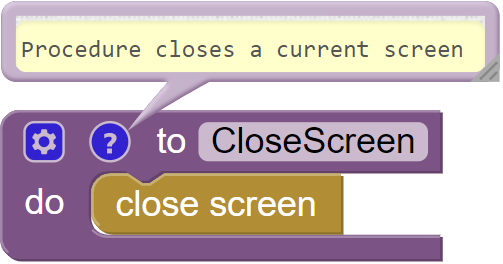
\includegraphics{./graphics/programs/guess_numbers/procedure_closeScreen_AppInventor_2018.png}
    \caption[Процедура CloseScreen.]{Процедура CloseScreen закрывает текущий экран.}
  \label{fig:block:click:close:screen}
\end{marginfigure}
Возникает вопрос: зачем действие по закрытию экрана помещать в отдельную процедуру? Это необходимо для того, чтобы последовательно выполнить блоки управления \textit{``open another screen''} и \textit{``close screen''} при возникновении события нажатия на любую навигационную кнопку (\textit{Click}). «Пазлы» блоков управления открытия и закрытия экрана спроектированы так, что их нельзя объединить в одном блоке App Inventor, но можно соединить их через вызов процедуры, что и было сделано (рис.~\ref{fig:block:click:close:screen}).

\chapter{Представление чисел}
\label{ch:need_to_think}

\newthought{Задача} заключается в следующем. Необходимо представить числа от 1 до 100 используя числа лишь одну выбранную цифру 
из набора 0...9, используя следующие математические операции: сложение, вычитание, умножение, деление, возведение в степень. 

\newthought{The front matter} of a book refers to all of the material that
comes before the main text.  The following table from shows a list of
material that appears in the front matter of \VDQI, \EI, \VE, and \BE
along with its page number.  Page numbers that appear in parentheses refer
to folios that do not have a printed page number (but they are still
counted in the page number sequence).



\chapter{Ответы}
\label{ch:answers}

\openepigraph{%
Ставлю три звездочки. 
Я видал в детских книжках: 
когда человек делает прыжок к новой мысли, он ставит три звездочки...
}{Саша Чёрный, {Дневник Фокса Микки}
}

\newthought{Задачи рассеяны} по всей книге, а ответы на них собраны в этом разделе.

\begin{task}
    \label{answer:Tricolor-flags}
    \newthought{Меняя порядок и толщину} горизонтальных полосок 
    сербского флага (с.~\pageref{fig:Srpska}), можно получить флаг России 
    или флаг Крыма (рис.~\ref{fig:FlagCrimea}). 
\end{task}

\begin{marginfigure}[0cm]
{%
\setlength{\fboxsep}{0pt}%
\setlength{\fboxrule}{1pt}%
\fcolorbox{gray}{gray}{
\includegraphics{./commons/Flag_of_Crimea.png}}%
}%
\caption{Флаг Крыма}
\label{fig:FlagCrimea}
\end{marginfigure}

\begin{task}
    \label{answer:Pobeda-beda}
    \newthought{Название корабля укоротилось} в мультфильме <<Приключения капитана 
    Врунгеля>>, поскольку юнга Лом срубил свежий лес для постройки яхты, поэтому корабль 
    и прирос к берегу. Пришлось рубить корни, первые две буквы не удержались и отвалились, 
    яхта <<Победа>> превратилась в <<Беду>>. 
    \small{Вопрос на с.~\pageref{fig:Pobeda-beda}.}
\end{task}

Задача: сколько ссылок можно закодировать, если ссылки содержит ровно 7 буквенно-цифровых символов,
     каждый символ может быть буквой английского алфавита 
     или цифрой от 0 до 9? Ответ на странице ... todo 

temp: Чем хороши глобальные переменные и какие у них недостатки
по сравнению с локальными переменными?

\begin{task}
    \label{answer:guess_numbers_task}
    \newthought{В алгоритме угадывания чисел} число $ a $ может быть натуральным, целым, вещественным и рациональным числом, то есть $ a \in \mathbb{N},\mathbb{Z}, \mathbb{Q}, \mathbb{R} $, но кроме иррациональных чисел из-за конечности разрядной сетки компьютера. 
    \small{Вопрос на с.~\pageref{question:text}}
\end{task}

\begin{task}
    \label{answer:global-vars-pros-cons}
    \newthought{Ответ такой} ... todo. 

    \small{Вопрос на с.~\pageref{fig:block:proc:swap:colors}.}
\end{task}



\chapter{The Design of Tufte's Books}
\label{ch:tufte-design}


\newthought{The pages} of a book are usually divided into three major
sections: the front matter (also called preliminary matter or prelim), the
main matter (the core text of the book), and the back matter (or end
matter).

\newthought{The front matter} of a book refers to all of the material that
comes before the main text.  The following table from shows a list of
material that appears in the front matter of \VDQI, \EI, \VE, and \BE
along with its page number.  Page numbers that appear in parentheses refer
to folios that do not have a printed page number (but they are still
counted in the page number sequence).

\bigskip
\begin{minipage}{\textwidth}
\begin{center}
\begin{tabular}{lcccc}
\toprule
 & \multicolumn{4}{c}{Books} \\
\cmidrule(l){2-5} 
Page content & \vdqi & \ei & \ve & \be \\
\midrule
Blank half title page & \hangp{1} & \hangp{1} & \hangp{1} & \hangp{1} \\
Frontispiece\footnotemark{}
  & \hangp{2} & \hangp{2} & \hangp{2} & \hangp{2} \\
Full title page & \hangp{3} & \hangp{3} & \hangp{3} & \hangp{3} \\
Copyright page & \hangp{4} & \hangp{4} & \hangp{4} & \hangp{4} \\
Contents & \hangp{5} & \hangp{5} & \hangp{5} & \hangp{5} \\
%Blank & -- & \hangp{6} & \hangp{6} & \hangp{6} \\
Dedication & \hangp{6} & \hangp{7} & \hangp{7} & 7 \\
%Blank & -- & \hangp{8} & -- & \hangp{8} \\
Epigraph & -- & -- & \hangp{8} & -- \\
Introduction & \hangp{7} & \hangp{9} & \hangp{9} & 9 \\
\bottomrule
\end{tabular}
\end{center}
\end{minipage}
\vspace{-7\baselineskip}\footnotetext{The contents of this page vary from book to book.  In
  \vdqi this page is blank; in \ei and \ve this page holds a frontispiece;
  and in \be this page contains three epigraphs.}
\vspace{7\baselineskip}

\bigskip
The design of the front matter in Tufte's books varies slightly from the
traditional design of front matter.  First, the pages in front matter are
traditionally numbered with lowercase roman numerals (e.g., i, ii, iii,
iv,~\ldots).  Second, the front matter page numbering sequence is usually
separate from the main matter page numbering.  That is, the page numbers
restart at 1 when the main matter begins.  In contrast, Tufte has
enumerated his pages with arabic numerals that share the same page counting
sequence as the main matter.  

There are also some variations in design across Tufte's four books.  The
page opposite the full title page (labeled ``frontispiece'' in the above
table) has different content in each of the books.  In \VDQI, this page is
blank; in \EI and \VE, this page holds a frontispiece; and in \BE, this
page contains three epigraphs.

The dedication appears on page~6 in \vdqi (opposite the introduction), and
is placed on its own spread in the other books.  In \ve, an epigraph shares
the spread with the opening page of the introduction.

None of the page numbers (folios) of the front matter are expressed except in
\be, where the folios start to appear on the dedication page.

\newthought{The full title page} of each of the books varies slightly in
design.  In all the books, the author's name appears at the top of the
page, the title it set just above the center line, and the publisher is
printed along the bottom margin.  Some of the differences are outlined in
the following table.

\bigskip
\begin{center}
\footnotesize
\begin{tabular}{lllll}
\toprule
Feature & \vdqi & \ei & \ve & \be \\
\midrule
Author & & & & \\
\quad Typeface & serif   & serif   & serif   & sans serif \\
\quad Style    & italics & italics & italics & upright, caps \\
\quad Size     & 24 pt   & 20 pt   & 20 pt   & 20 pt \\
\addlinespace
Title & & & & \\
\quad Typeface & serif   & serif   & serif   & sans serif \\
\quad Style    & upright & italics & upright & upright, caps \\
\quad Size     & 36 pt   & 48 pt   & 48 pt   & 36 pt \\
\addlinespace
Subtitle & & & & \\
\quad Typeface & \na     & \na     & serif   & \na \\
\quad Style    & \na     & \na     & upright & \na \\
\quad Size     & \na     & \na     & 20 pt   & \na \\
\addlinespace
Edition & & & & \\
\quad Typeface & sans serif    & \na  & \na  & \na \\
\quad Style    & upright, caps & \na  & \na  & \na \\
\quad Size     & 14 pt         & \na  & \na  & \na \\
\addlinespace
Publisher & & & & \\
\quad Typeface & serif   & serif   & serif   & sans serif \\
\quad Style    & italics & italics & italics & upright, caps \\
\quad Size     & 14 pt   & 14 pt   & 14 pt   & 14 pt \\
\bottomrule
\end{tabular}
\end{center}

\begin{figure*}[p]
\fbox{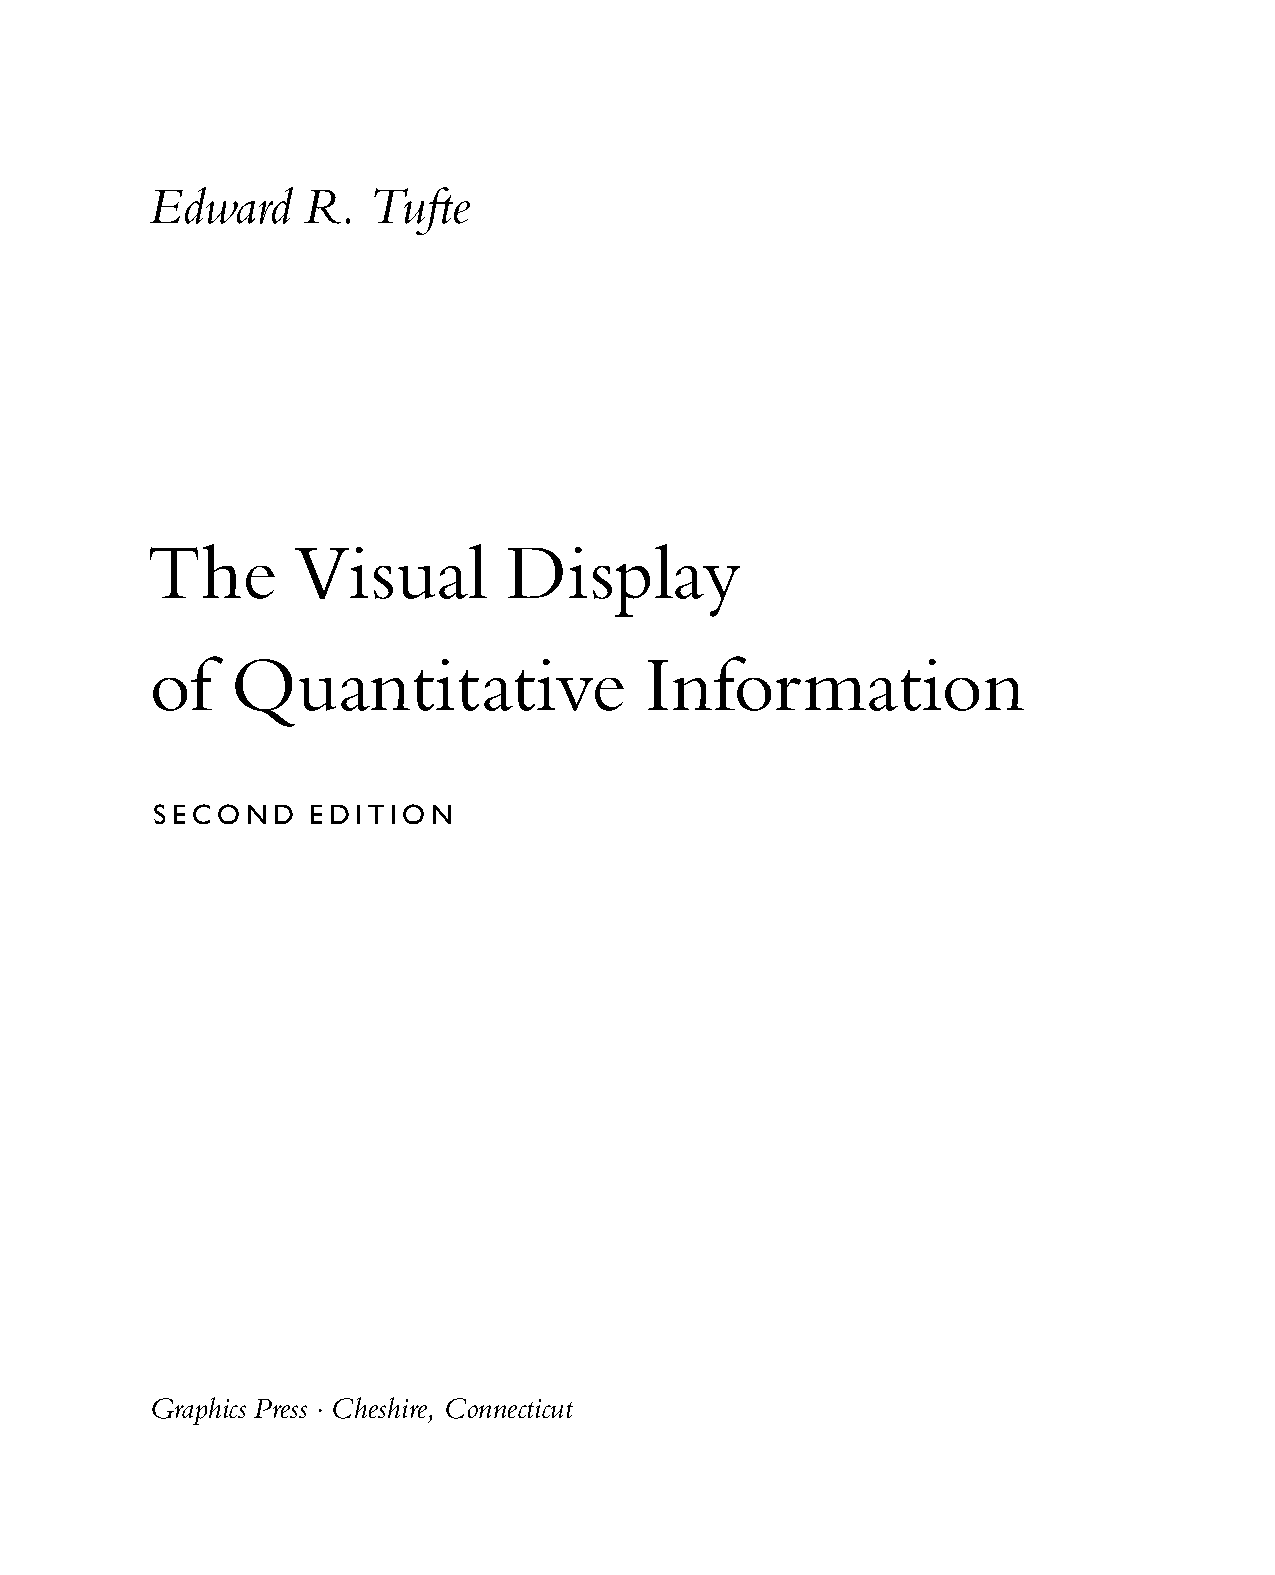
\includegraphics[width=0.45\linewidth]{graphics/temp/vdqi-title.pdf}}
\hfill
\fbox{
\includegraphics[width=0.45\linewidth]{graphics/temp/ei-title.pdf}}
\\\vspace{\baselineskip}
\fbox{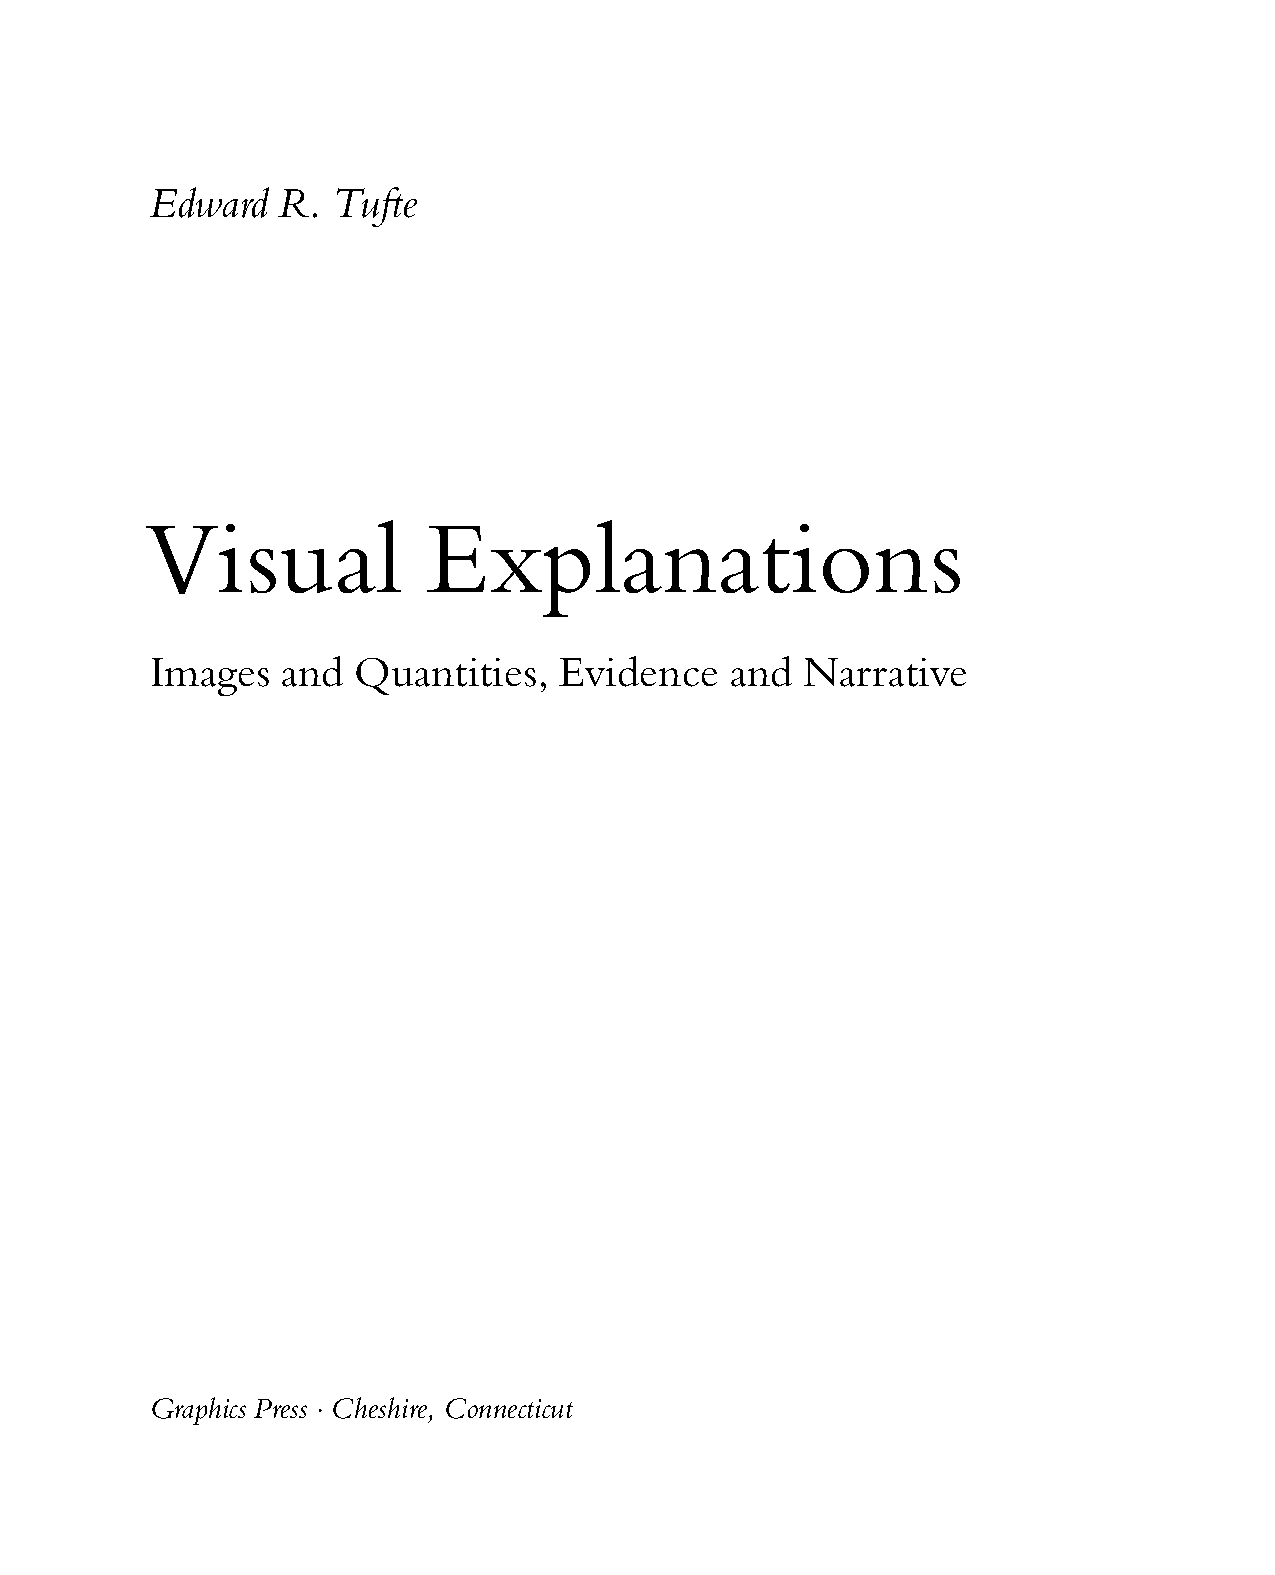
\includegraphics[width=0.45\linewidth]{graphics/temp/ve-title.pdf}}
\hfill
\fbox{
\includegraphics[width=0.45\linewidth]{graphics/temp/be-title.pdf}}
\end{figure*}

\newthought{The tables of contents} in Tufte's books give us our first
glimpse of the structure of the main matter.  \VDQI is split into two
parts, each containing some number of chapters.  His other three books only
contain chapters---they're not broken into parts.

\begin{figure*}[p]\index{table of contents}
\fbox{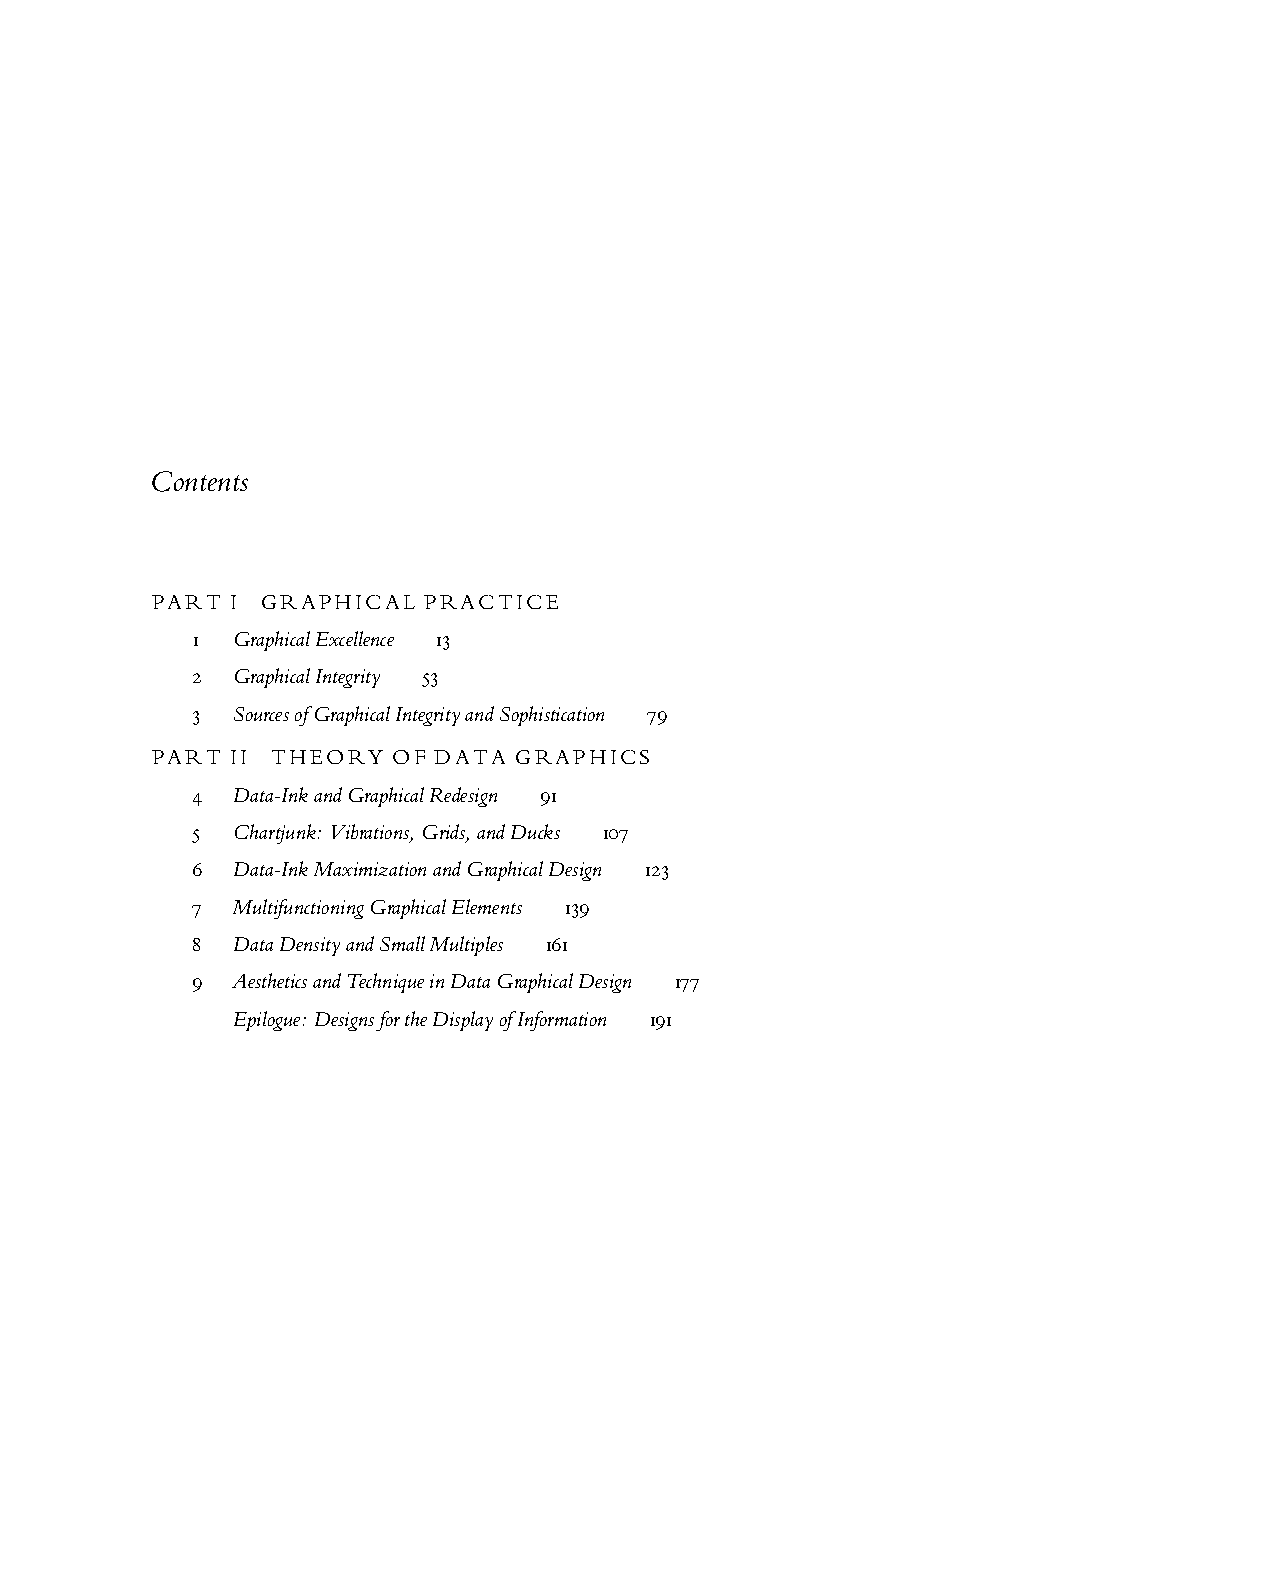
\includegraphics[width=0.45\linewidth]{graphics/temp/vdqi-contents.pdf}}
\hfill
\fbox{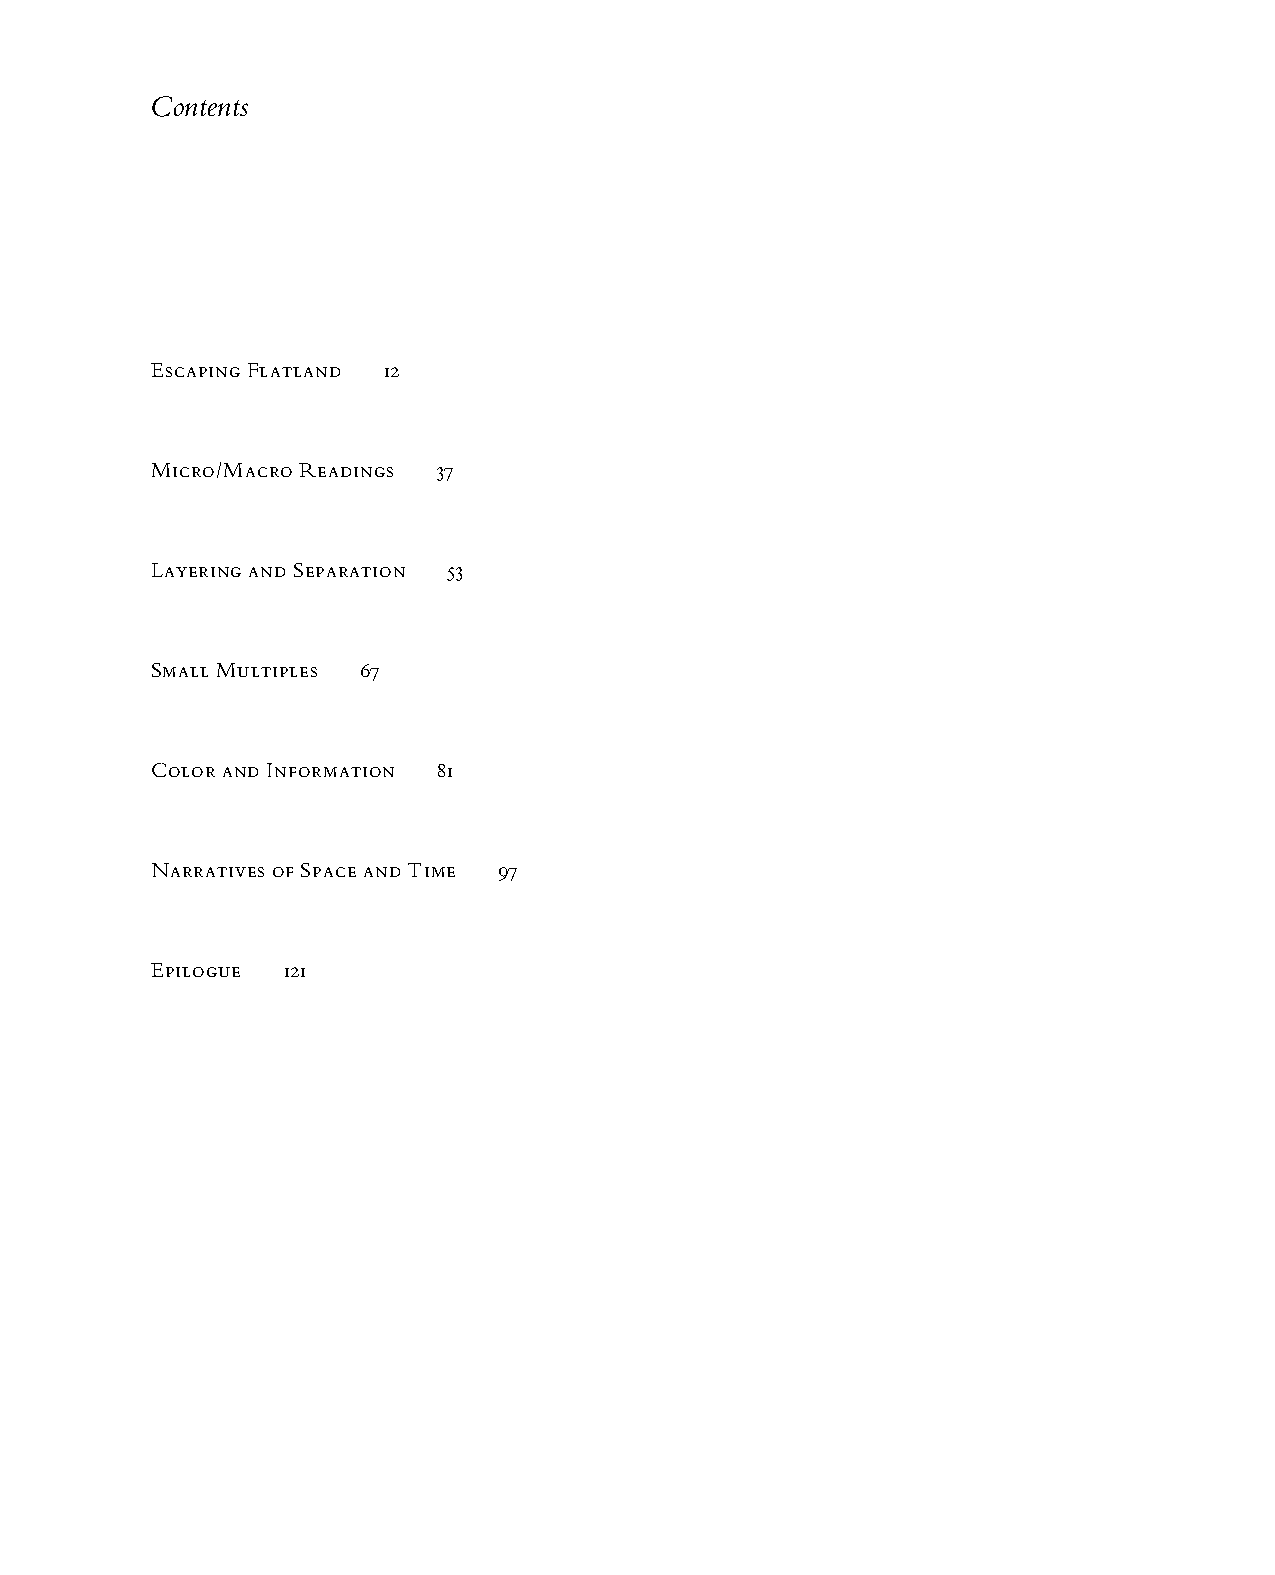
\includegraphics[width=0.45\linewidth]{graphics/temp/ei-contents.pdf}}
\\\vspace{\baselineskip}
\fbox{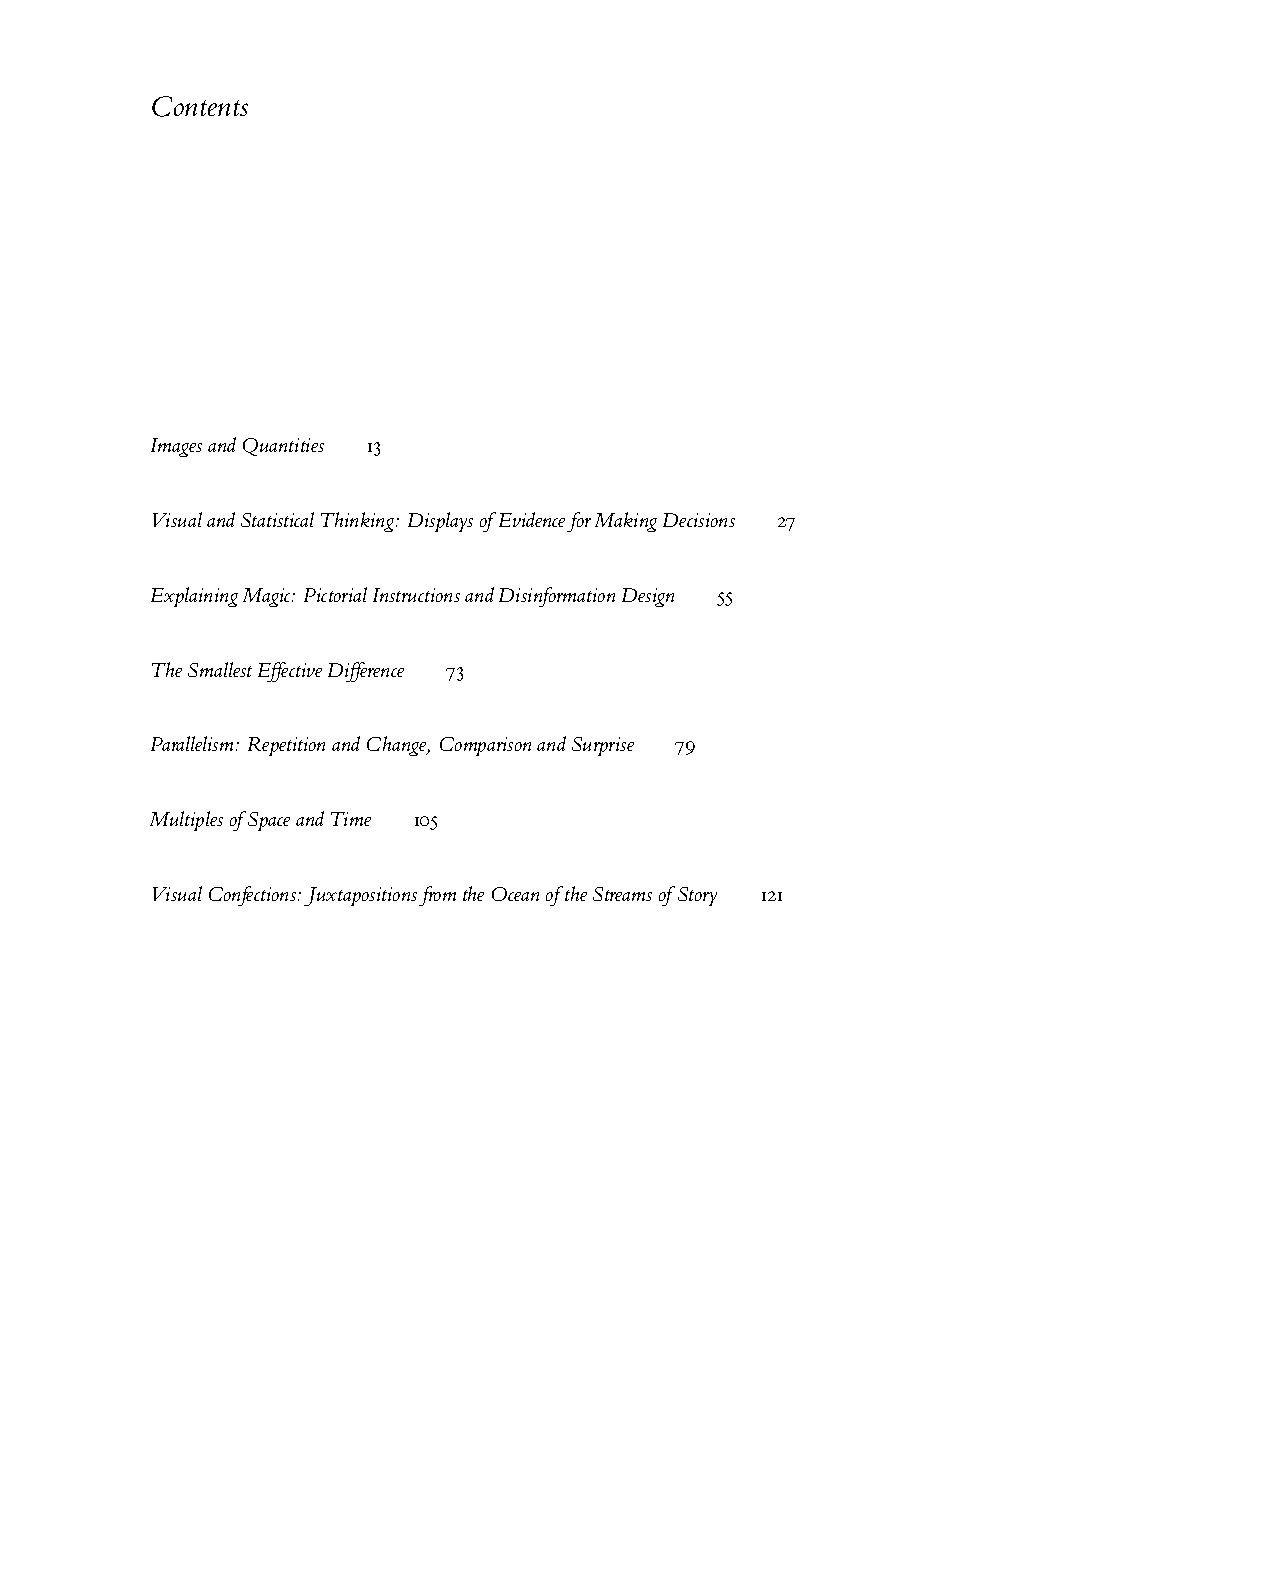
\includegraphics[width=0.45\linewidth]{graphics/temp/ve-contents.pdf}}
\hfill
\fbox{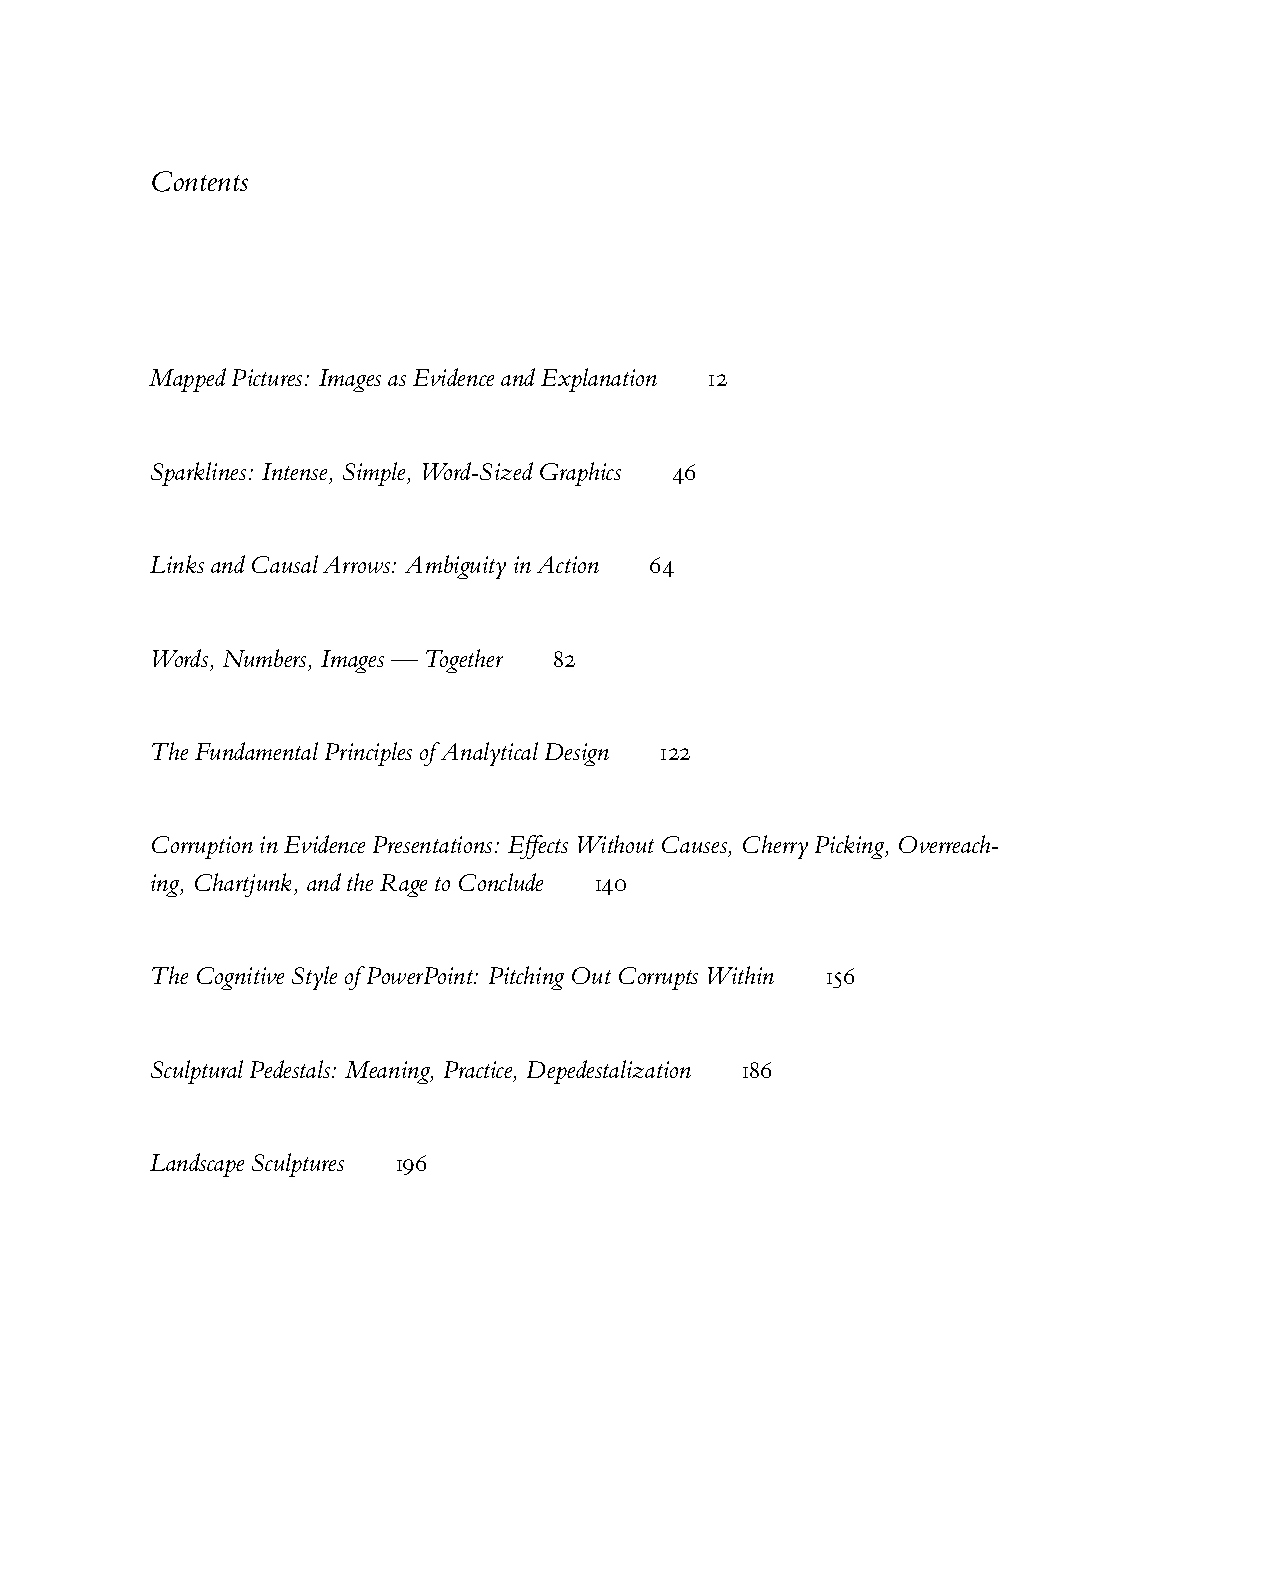
\includegraphics[width=0.45\linewidth]{graphics/temp/be-contents.pdf}}
\end{figure*}


\section{Typefaces}\label{sec:typefaces1}\index{typefaces}
\index{fonts|see{typefaces}}

Tufte's books primarily use two typefaces: Bembo and Gill Sans.  Bembo is used
for the headings and body text, while Gill Sans is used for the title page and
opening epigraphs in \BE.

Since neither Bembo nor Gill Sans are available in default \LaTeX{}
installations, the \TL document classes default to using Palatino and
Helvetica, respectively.  In addition, the Bera Mono typeface is used for
\texttt{monospaced} type.

The following font sizes are defined by the \TL classes:

\begin{table}[h]\index{typefaces!sizes}
  \footnotesize%
  \begin{center}
    \begin{tabular}{lccl}
      \toprule
      \LaTeX{} size & Font size & Leading & Used for \\
      \midrule
      \verb+\tiny+         &  5 &  6 & sidenote numbers \\
      \verb+\scriptsize+   &  7 &  8 & \na \\
      \verb+\footnotesize+ &  8 & 10 & sidenotes, captions \\
      \verb+\small+        &  9 & 12 & quote, quotation, and verse environments \\
      \verb+\normalsize+   & 10 & 14 & body text \\
      \verb+\large+        & 11 & 15 & \textsc{b}-heads \\
      \verb+\Large+        & 12 & 16 & \textsc{a}-heads, \textsc{toc} entries, author, date \\
      \verb+\LARGE+        & 14 & 18 & handout title \\
      \verb+\huge+         & 20 & 30 & chapter heads \\
      \verb+\Huge+         & 24 & 36 & part titles \\
      \bottomrule
    \end{tabular}
  \end{center}
  \caption{A list of \LaTeX{} font sizes as defined by the \TL document classes.}
  \label{tab:font-sizes}
\end{table}

\section{Headings}\label{sec:headings1}\index{headings}

Tufte's books include the following heading levels: parts,
chapters,\sidenote{Parts and chapters are defined for the \texttt{tufte-book}
class only.}  sections, subsections, and paragraphs.  Not defined by default
are: sub-subsections and subparagraphs.

\begin{table}[h]
  \begin{center}
    \footnotesize%
    \begin{tabular}{lcr}
      \toprule
      Heading & Style & Size \\
      \midrule
      Part & roman & \measure{24}{36}{40} \\
      Chapter & italic & \measure{20}{30}{40} \\
      Section & italic & \measure{12}{16}{26} \\
      Subsection & italic & \measure{11}{15}{26} \\
      Paragraph & italic & 10/14 \\
      \bottomrule
    \end{tabular}
  \end{center}
  \caption{Heading styles used in \BE.}
  \label{tab:heading-styles}
\end{table}

\paragraph{Paragraph} Paragraph headings (as shown here) are introduced by
italicized text and separated from the main paragraph by a bit of space.

\section{Environments}

The following characteristics define the various environments:


\begin{table}[h]
  \begin{center}
    \footnotesize%
    \begin{tabular}{lcl}
      \toprule
      Environment & Font size & Notes \\
      \midrule
      Body text & \measure{10}{14}{26} & \\
      Block quote & \measure{9}{12}{24} & Block indent (left and right) by \unit[1]{pc} \\
      Sidenotes & \measure{8}{10}{12} & Sidenote number is set inline, followed by word space \\
      Captions & \measure{8}{10}{12} &  \\
      \bottomrule
    \end{tabular}
  \end{center}
  \caption{Environment styles used in \BE.}
  \label{tab:environment-styles}
\end{table}


\chapter[On the Use of the tufte-book Document Class]{On the Use of the \texttt{tufte-book} Document Class}
\label{ch:tufte-book}

The \TL document classes define a style similar to the
style Edward Tufte uses in his books and handouts.  Tufte's style is known
for its extensive use of sidenotes, tight integration of graphics with
text, and well-set typography.  This document aims to be at once a
demonstration of the features of the \TL document classes
and a style guide to their use.

\section{Page Layout}\label{sec:page-layout}
\subsection{Headings}\label{sec:headings}\index{headings}
This style provides \textsc{a}- and \textsc{b}-heads (that is,
\Verb|\section| and \Verb|\subsection|), demonstrated above.

If you need more than two levels of section headings, you'll have to define
them yourself at the moment; there are no pre-defined styles for anything below
a \Verb|\subsection|.  

The \TL classes will emit an error if you try to use
\linebreak\Verb|\subsubsection| and smaller headings.

% let's start a new thought -- a new section
\newthought{In his later books},\cite{Galanin} Tufte
starts each section with a bit of vertical space, a non-indented paragraph,
and sets the first few words of the sentence in \textsc{small caps}.  To
accomplish this using this style, use the \doccmddef{newthought} command:
\begin{docspec}
  \doccmd{newthought}\{In his later books\}, Tufte starts\ldots
\end{docspec}


\section{Sidenotes}\label{sec:sidenotes}
One of the most prominent and distinctive features of this style is the
extensive use of sidenotes.  There is a wide margin to provide ample room
for sidenotes and small figures.  Any \doccmd{footnote}s will automatically
be converted to sidenotes.\footnote{This is a sidenote that was entered
using the \texttt{\textbackslash footnote} command.}  If you'd like to place ancillary
information in the margin without the sidenote mark (the superscript
number), you can use the \doccmd{marginnote} command.\marginnote{This is a
margin note.  Notice that there isn't a number preceding the note, and
there is no number in the main text where this note was written.}

The specification of the \doccmddef{sidenote} command is:
\begin{docspec}
  \doccmd{sidenote}[\docopt{number}][\docopt{offset}]\{\docarg{Sidenote text.}\}
\end{docspec}

Both the \docopt{number} and \docopt{offset} arguments are optional.  If you
provide a \docopt{number} argument, then that number will be used as the
sidenote number.  It will change the number of the current sidenote only and
will not affect the numbering sequence of subsequent sidenotes.

Sometimes a sidenote may run over the top of other text or graphics in the
margin space.  If this happens, you can adjust the vertical position of the
sidenote by providing a dimension in the \docopt{offset} argument.  Some
examples of valid dimensions are:
\begin{docspec}
  \ttfamily 1.0in \qquad 2.54cm \qquad 254mm \qquad 6\Verb|\baselineskip|
\end{docspec}
If the dimension is positive it will push the sidenote down the page; if the
dimension is negative, it will move the sidenote up the page.

While both the \docopt{number} and \docopt{offset} arguments are optional, they
must be provided in order.  To adjust the vertical position of the sidenote
while leaving the sidenote number alone, use the following syntax:
\begin{docspec}
  \doccmd{sidenote}[][\docopt{offset}]\{\docarg{Sidenote text.}\}
\end{docspec}
The empty brackets tell the \Verb|\sidenote| command to use the default
sidenote number.

If you \emph{only} want to change the sidenote number, however, you may
completely omit the \docopt{offset} argument:
\begin{docspec}
  \doccmd{sidenote}[\docopt{number}]\{\docarg{Sidenote text.}\}
\end{docspec}

The \doccmddef{marginnote} command has a similar \docarg{offset} argument:
\begin{docspec}
  \doccmd{marginnote}[\docopt{offset}]\{\docarg{Margin note text.}\}
\end{docspec}

\section{References}
References are placed alongside their citations as sidenotes,
as well.  This can be accomplished using the normal \doccmddef{cite}
command.\sidenote{The first paragraph of this document includes a citation.}

The complete list of references may also be printed automatically by using
the \doccmddef{bibliography} command.  (See the end of this document for an
example.)  If you do not want to print a bibliography at the end of your
document, use the \doccmddef{nobibliography} command in its place.  

To enter multiple citations at one location,\cite[-3\baselineskip]{Galanin,KamrianiAndRoy2016} you can
provide a list of keys separated by commas and the same optional vertical
offset argument: \Verb|\cite{Galanin,KamrianiAndRoy2016}|.  
\begin{docspec}
  \doccmd{cite}[\docopt{offset}]\{\docarg{bibkey1,bibkey2,\ldots}\}
\end{docspec}

\section{Figures and Tables}\label{sec:figures-and-tables}
Images and graphics play an integral role in Tufte's work.
In addition to the standard \docenvdef{figure} and \docenvdef{tabular} environments,
this style provides special figure and table environments for full-width
floats.

Full page--width figures and tables may be placed in \docenvdef{figure*} or
\docenvdef{table*} environments.  To place figures or tables in the margin,
use the \docenvdef{marginfigure} or \docenvdef{margintable} environments as follows
(see figure~\ref{fig:marginfig}):

\begin{marginfigure}%
  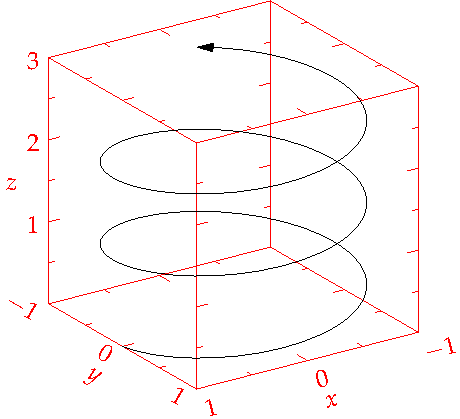
\includegraphics[width=\linewidth]{temp/helix}
  \caption{This is a margin figure.  The helix is defined by 
    $x = \cos(2\pi z)$, $y = \sin(2\pi z)$, and $z = [0, 2.7]$.  The figure was
    drawn using Asymptote (\url{http://asymptote.sf.net/}).}
  \label{fig:marginfig}
\end{marginfigure}

\begin{docspec}
\textbackslash begin\{marginfigure\}\\
  \qquad\textbackslash includegraphics\{temp/helix\}\\
  \qquad\textbackslash caption\{This is a margin figure.\}\\
  \qquad\textbackslash label\{fig:marginfig\}\\
\textbackslash end\{marginfigure\}\\
\end{docspec}

The \docenv{marginfigure} and \docenv{margintable} environments accept an optional parameter \docopt{offset} that adjusts the vertical position of the figure or table.  See the ``\nameref{sec:sidenotes}'' section above for examples.  The specifications are:
\begin{docspec}
  \textbackslash{begin\{marginfigure\}[\docopt{offset}]}\\
  \qquad\ldots\\
  \textbackslash{end\{marginfigure\}}\\
  \mbox{}\\
  \textbackslash{begin\{margintable\}[\docopt{offset}]}\\
  \qquad\ldots\\
  \textbackslash{end\{margintable\}}\\
\end{docspec}

Figure~\ref{fig:fullfig} is an example of the \docenv{figure*}
environment and figure~\ref{fig:textfig} is an example of the normal
\docenv{figure} environment.

\begin{figure*}[h]
  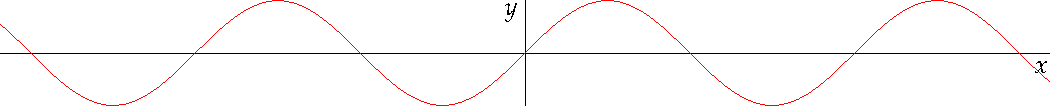
\includegraphics[width=\linewidth]{temp/sine.pdf}%
  \caption{This graph shows $y = \sin x$ from about $x = [-10, 10]$.
  \emph{Notice that this figure takes up the full page width.}}%
  \label{fig:fullfig}%
\end{figure*}

\begin{figure}
  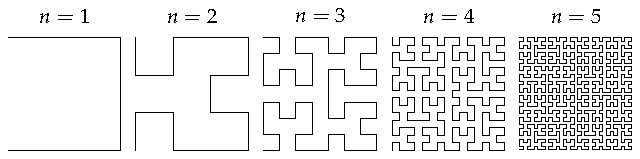
\includegraphics{temp/hilbertcurves.pdf}
%  \checkparity This is an \pageparity\ page.%
  \caption[Hilbert curves of various degrees $n$.][6pt]{Hilbert curves of various degrees $n$. \emph{Notice that this figure only takes up the main textblock width.}}
  \label{fig:textfig}
  %\zsavepos{pos:textfig}
\end{figure}

As with sidenotes and marginnotes, a caption may sometimes require vertical
adjustment. The \doccmddef{caption} command now takes a second optional
argument that enables you to do this by providing a dimension \docopt{offset}.
You may specify the caption in any one of the following forms:
\begin{docspec}
  \doccmd{caption}\{\docarg{long caption}\}\\
  \doccmd{caption}[\docarg{short caption}]\{\docarg{long caption}\}\\
  \doccmd{caption}[][\docopt{offset}]\{\docarg{long caption}\}\\
  \doccmd{caption}[\docarg{short caption}][\docopt{offset}]%
                  \{\docarg{long caption}\}
\end{docspec}
A positive \docopt{offset} will push the caption down the page. The short
caption, if provided, is what appears in the list of figures/tables, otherwise
the ``long'' caption appears there. Note that although the arguments
\docopt{short caption} and \docopt{offset} are both optional, they must be
provided in order. Thus, to specify an \docopt{offset} without specifying a
\docopt{short caption}, you must include the first set of empty brackets
\Verb|[]|, which tell \doccmd{caption} to use the default ``long'' caption. As
an example, the caption to figure~\ref{fig:textfig} above was given in the form
\begin{docspec}
  \doccmd{caption}[Hilbert curves...][6pt]\{Hilbert curves...\}
\end{docspec}

Table~\ref{tab:normaltab} shows table created with the \docpkg{booktabs}
package.  Notice the lack of vertical rules---they serve only to clutter
the table's data.

\begin{table}[ht]
  \centering
  \fontfamily{ppl}\selectfont
  \begin{tabular}{ll}
    \toprule
    Margin & Length \\
    \midrule
    Paper width & \unit[8\nicefrac{1}{2}]{inches} \\
    Paper height & \unit[11]{inches} \\
    Textblock width & \unit[6\nicefrac{1}{2}]{inches} \\
    Textblock/sidenote gutter & \unit[\nicefrac{3}{8}]{inches} \\
    Sidenote width & \unit[2]{inches} \\
    \bottomrule
  \end{tabular}
  \caption{Here are the dimensions of the various margins used in the Tufte-handout class.}
  \label{tab:normaltab}
  %\zsavepos{pos:normaltab}
\end{table}

\newthought{Occasionally} \LaTeX{} will generate an error message:\label{err:too-many-floats}
\begin{docspec}
  Error: Too many unprocessed floats
\end{docspec}
\LaTeX{} tries to place floats in the best position on the page.  Until it's
finished composing the page, however, it won't know where those positions are.
If you have a lot of floats on a page (including sidenotes, margin notes,
figures, tables, etc.), \LaTeX{} may run out of ``slots'' to keep track of them
and will generate the above error.

\LaTeX{} initially allocates 18 slots for storing floats.  To work around this
limitation, the \TL document classes provide a \doccmddef{morefloats} command
that will reserve more slots.

The first time \doccmd{morefloats} is called, it allocates an additional 34
slots.  The second time \doccmd{morefloats} is called, it allocates another 26
slots.

The \doccmd{morefloats} command may only be used two times.  Calling it a
third time will generate an error message.  (This is because we can't safely
allocate many more floats or \LaTeX{} will run out of memory.)

If, after using the \doccmd{morefloats} command twice, you continue to get the
\texttt{Too many unprocessed floats} error, there are a couple things you can
do.

The \doccmddef{FloatBarrier} command will immediately process all the floats
before typesetting more material.  Since \doccmd{FloatBarrier} will start a new
paragraph, you should place this command at the beginning or end of a
paragraph.

The \doccmddef{clearpage} command will also process the floats before
continuing, but instead of starting a new paragraph, it will start a new page.

You can also try moving your floats around a bit: move a figure or table to the
next page or reduce the number of sidenotes.  (Each sidenote actually uses
\emph{two} slots.)

After the floats have placed, \LaTeX{} will mark those slots as unused so they
are available for the next page to be composed.

\section{Captions}
You may notice that the captions are sometimes misaligned.
Due to the way \LaTeX's float mechanism works, we can't know for sure where it
decided to put a float. Therefore, the \TL document classes provide commands to
override the caption position.

\paragraph{Vertical alignment} To override the vertical alignment, use the
\doccmd{setfloatalignment} command inside the float environment.  For
example:

\begin{fullwidth}
\begin{docspec}
  \textbackslash begin\{figure\}[btp]\\
  \qquad \textbackslash includegraphics\{sinewave\}\\
  \qquad \textbackslash caption\{This is an example of a sine wave.\}\\
  \qquad \textbackslash label\{fig:sinewave\}\\
  \qquad \hlred{\textbackslash setfloatalignment\{b\}\% forces caption to be bottom-aligned}\\
  \textbackslash end\{figure\}
\end{docspec}
\end{fullwidth}

\noindent The syntax of the \doccmddef{setfloatalignment} command is:

\begin{docspec}
  \doccmd{setfloatalignment}\{\docopt{pos}\}
\end{docspec}

\noindent where \docopt{pos} can be either \texttt{b} for bottom-aligned
captions, or \texttt{t} for top-aligned captions.

\paragraph{Horizontal alignment}\label{par:overriding-horizontal}
To override the horizontal alignment, use either the \doccmd{forceversofloat}
or the \doccmd{forcerectofloat} command inside of the float environment.  For
example:

\begin{fullwidth}
\begin{docspec}
  \textbackslash begin\{figure\}[btp]\\
  \qquad \textbackslash includegraphics\{sinewave\}\\
  \qquad \textbackslash caption\{This is an example of a sine wave.\}\\
  \qquad \textbackslash label\{fig:sinewave\}\\
  \qquad \hlred{\textbackslash forceversofloat\% forces caption to be set to the left of the float}\\
  \textbackslash end\{figure\}
\end{docspec}
\end{fullwidth}

The \doccmddef{forceversofloat} command causes the algorithm to assume the
float has been placed on a verso page---that is, a page on the left side of a
two-page spread.  Conversely, the \doccmddef{forcerectofloat} command causes
the algorithm to assume the float has been placed on a recto page---that is, a
page on the right side of a two-page spread.


\section{Full-width text blocks}

In addition to the new float types, there is a \docenvdef{fullwidth}
environment that stretches across the main text block and the sidenotes
area.

\begin{Verbatim}
\begin{fullwidth}
Lorem ipsum dolor sit amet...
\end{fullwidth}
\end{Verbatim}

\begin{fullwidth}
\small\itshape\lipsum[1]
\end{fullwidth}

\section{Typography}\label{sec:typography}

\subsection{Typefaces}\label{sec:typefaces}\index{typefaces}
If the Palatino, \textsf{Helvetica}, and \texttt{Bera Mono} typefaces are installed, this style
will use them automatically.  Otherwise, we'll fall back on the Computer Modern
typefaces.

\subsection{Letterspacing}\label{sec:letterspacing}
This document class includes two new commands and some improvements on
existing commands for letterspacing.

When setting strings of \allcaps{ALL CAPS} or \smallcaps{small caps}, the
letter\-spacing---that is, the spacing between the letters---should be
increased slightly.  The \doccmddef{allcaps} command has proper letterspacing for
strings of \allcaps{FULL CAPITAL LETTERS}, and the \doccmddef{smallcaps} command
has letterspacing for \smallcaps{small capital letters}.  These commands
will also automatically convert the case of the text to upper- or
lowercase, respectively.

The \doccmddef{textsc} command has also been redefined to include
letterspacing.  The case of the \doccmd{textsc} argument is left as is,
however.  This allows one to use both uppercase and lowercase letters:
\textsc{The Initial Letters Of The Words In This Sentence Are Capitalized.}



\section{Document Class Options}\label{sec:options}

\index{class options|(}
The \doccls{tufte-book} class is based on the \LaTeX\ \doccls{book}
document class.  Therefore, you can pass any of the typical book
options.  There are a few options that are specific to the
\doccls{tufte-book} document class, however.

The \docclsoptdef{a4paper} option will set the paper size to \smallcaps{A4} instead of
the default \smallcaps{US} letter size.

The \docclsoptdef{sfsidenotes} option will set the sidenotes and title block in a 
\textsf{sans serif} typeface instead of the default roman.

The \docclsoptdef{twoside} option will modify the running heads so that the page
number is printed on the outside edge (as opposed to always printing the page
number on the right-side edge in \docclsoptdef{oneside} mode).  

The \docclsoptdef{symmetric} option typesets the sidenotes on the outside edge of
the page.  This is how books are traditionally printed, but is contrary to
Tufte's book design which sets the sidenotes on the right side of the page.
This option implicitly sets the \docclsopt{twoside} option.

The \docclsoptdef{justified} option sets all the text fully justified (flush left
and right).  The default is to set the text ragged right.  
The body text of Tufte's books are set ragged right.  This prevents
needless hyphenation and makes it easier to read the text in the slightly
narrower column.

The \docclsoptdef{bidi} option loads the \docpkg{bidi} package which is used with
\tXeLaTeX\ to typeset bi-directional text.  Since the \docpkg{bidi}
package needs to be loaded before the sidenotes and cite commands are defined,
it can't be loaded in the document preamble.

The \docclsoptdef{debug} option causes the \TL classes to output debug
information to the log file which is useful in troubleshooting bugs.  It will
also cause the graphics to be replaced by outlines.

The \docclsoptdef{nofonts} option prevents the \TL classes from
automatically loading the Palatino and Helvetica typefaces.  You should use
this option if you wish to load your own fonts.  If you're using \tXeLaTeX, this
option is implied (i.e., the Palatino and Helvetica fonts aren't loaded if you
use \tXeLaTeX).  

The \docclsoptdef{nols} option inhibits the letterspacing code.  The \TL\
classes try to load the appropriate letterspacing package (either pdf\TeX's
\docpkg{letterspace} package or the \docpkg{soul} package).  If you're using
\tXeLaTeX\ with \docpkg{fontenc}, however, you should configure your own
letterspacing.  

The \docclsoptdef{notitlepage} option causes \doccmd{maketitle} to generate a title
block instead of a title page.  The \doccls{book} class defaults to a title
page and the \doccls{handout} class defaults to the title block.  There is an
analogous \docclsoptdef{titlepage} option that forces \doccmd{maketitle} to
generate a full title page instead of the title block.

The \docclsoptdef{notoc} option suppresses \TL's custom table of contents
(\textsc{toc}) design.  The current \textsc{toc} design only shows unnumbered
chapter titles; it doesn't show sections or subsections.  The \docclsopt{notoc}
option will revert to \LaTeX's \textsc{toc} design.

The \docclsoptdef{nohyper} option prevents the \docpkg{hyperref} package from
being loaded.  The default is to load the \docpkg{hyperref} package and use the
\doccmd{title} and \doccmd{author} contents as metadata for the generated
\textsc{pdf}.

\index{class options|)}



\chapter[Customizing Tufte-LaTeX]{Customizing \TL}
\label{ch:customizing}

The \TL document classes are designed to closely emulate Tufte's book
design by default.  However, each document is different and you may encounter
situations where the default settings are insufficient.  This chapter explores
many of the ways you can adjust the \TL document classes to better fit
your needs.

\section{File Hooks}
\label{sec:filehooks}

\index{file hooks|(}
If you create many documents using the \TL classes, it's easier to
store your customizations in a separate file instead of copying them into the
preamble of each document.  The \TL classes provide three file hooks:
\docfilehook{tufte-common-local.tex}{common}, \docfilehook{tufte-book-local.tex}{book}, and
\docfilehook{tufte-handout-local.tex}{handout}.\sloppy

\begin{description}
  \item[\docfilehook{tufte-common-local.tex}{common}]
    If this file exists, it will be loaded by all of the \TL document
    classes just prior to any document-class-specific code.  If your
    customizations or code should be included in both the book and handout
    classes, use this file hook.
  \item[\docfilehook{tufte-book-local.tex}{book}] 
    If this file exists, it will be loaded after all of the common and
    book-specific code has been read.  If your customizations apply only to the
    book class, use this file hook.
  \item[\docfilehook{tufte-common-handout.tex}{handout}] 
    If this file exists, it will be loaded after all of the common and
    handout-specific code has been read.  If your customizations apply only to
    the handout class, use this file hook.
\end{description}

\index{file hooks|)}

\section{Numbered Section Headings}
\label{sec:numbered-sections}
\index{headings!numbered}

While Tufte dispenses with numbered headings in his books, if you require them,
they can be anabled by changing the value of the \doccounter{secnumdepth}
counter.  From the table below, select the heading level at which numbering
should stop and set the \doccounter{secnumdepth} counter to that value.  For
example, if you want parts and chapters numbered, but don't want numbering for
sections or subsections, use the command:
\begin{docspec}
  \doccmd{setcounter}\{secnumdepth\}\{0\}
\end{docspec}

The default \doccounter{secnumdepth} for the \TL document classes is $-1$.

\begin{table}
  \footnotesize
  \begin{center}
    \begin{tabular}{lr}
      \toprule
      Heading level & Value \\
      \midrule
      Part (in \doccls{tufte-book}) & $-1$ \\
      Part (in \doccls{tufte-handout}) & $0$ \\
      Chapter (only in \doccls{tufte-book}) & $0$ \\
      Section & $1$ \\
      Subsection & $2$ \\
      Subsubsection & $3$ \\
      Paragraph & $4$ \\
      Subparagraph & $5$ \\
      \bottomrule
    \end{tabular}
  \end{center}
  \caption{Heading levels used with the \texttt{secnumdepth} counter.}
\end{table}

\section{Changing the Paper Size}
\label{sec:paper-size}

The \TL classes currently only provide three paper sizes: \textsc{a4},
\textsc{b5}, and \textsc{us} letter.  To specify a different paper size (and/or
margins), use the \doccmd[geometry]{geometry} command in the preamble of your
document (or one of the file hooks).  The full documentation of the
\doccmd{geometry} command may be found in the \docpkg{geometry} package
documentation.


\section{Customizing Marginal Material}
\label{sec:marginal-material}

Marginal material includes sidenotes, citations, margin notes, and captions.
Normally, the justification of the marginal material follows the justification
of the body text.  If you specify the \docclsopt{justified} document class
option, all of the margin material will be fully justified as well.  If you
don't specify the \docclsopt{justified} option, then the marginal material will
be set ragged right.

You can set the justification of the marginal material separately from the body
text using the following document class options: \docclsopt{sidenote},
\docclsopt{marginnote}, \docclsopt{caption}, \docclsopt{citation}, and
\docclsopt{marginals}.  Each option refers to its obviously corresponding
marginal material type.  The \docclsopt{marginals} option simultaneously sets
the justification on all four marginal material types.

Each of the document class options takes one of five justification types:
\begin{description}
  \item[\docclsopt{justified}] Fully justifies the text (sets it flush left and
    right).
  \item[\docclsopt{raggedleft}] Sets the text ragged left, regardless of which
    page it falls on.
  \item[\docclsopt{raggedright}] Sets the text ragged right, regardless of
    which page it falls on.
  \item[\doccls{raggedouter}] Sets the text ragged left if it falls on the
    left-hand (verso) page of the spread and otherwise sets it ragged right.
    This is useful in conjunction with the \docclsopt{symmetric} document class
    option.
  \item[\docclsopt{auto}] If the \docclsopt{justified} document class option
    was specified, then set the text fully justified; otherwise the text is set
    ragged right.  This is the default justification option if one is not
    explicitly specified.
\end{description}

\noindent For example, 
\begin{docspec}
  \doccmdnoindex{documentclass}[symmetric,justified,marginals=raggedouter]\{tufte-book\}
\end{docspec}
will set the body text of the document to be fully justified and all of the
margin material (sidenotes, margin notes, captions, and citations) to be flush
against the body text with ragged outer edges.

\newthought{The font and style} of the marginal material may also be modified using the following commands:

\begin{docspec}
  \doccmd{setsidenotefont}\{\docopt{font commands}\}\\
  \doccmd{setcaptionfont}\{\docopt{font commands}\}\\
  \doccmd{setmarginnotefont}\{\docopt{font commands}\}\\
  \doccmd{setcitationfont}\{\docopt{font commands}\}
\end{docspec}

The \doccmddef{setsidenotefont} sets the font and style for sidenotes, the
\doccmddef{setcaptionfont} for captions, the \doccmddef{setmarginnotefont} for
margin notes, and the \doccmddef{setcitationfont} for citations.  The
\docopt{font commands} can contain font size changes (e.g.,
\doccmdnoindex{footnotesize}, \doccmdnoindex{Huge}, etc.), font style changes (e.g.,
\doccmdnoindex{sffamily}, \doccmdnoindex{ttfamily}, \doccmdnoindex{itshape}, etc.), color changes (e.g.,
\doccmdnoindex{color}\texttt{\{blue\}}), and many other adjustments.

If, for example, you wanted the captions to be set in italic sans serif, you could use:
\begin{docspec}
  \doccmd{setcaptionfont}\{\doccmdnoindex{itshape}\doccmdnoindex{sffamily}\}
\end{docspec}

\chapter{Compatibility Issues}
\label{ch:compatibility}

When switching an existing document from one document class to a \TL document class, a few changes to the document may have to be made.

\section{Converting from \doccls{article} to \doccls{tufte-handout}}

The following \doccls{article} class options are unsupported: \docclsopt{10pt}, \docclsopt{11pt}, \docclsopt{12pt}, \docclsopt{a5paper}, \docclsopt{b5paper}, \docclsopt{executivepaper}, \docclsopt{legalpaper}, \docclsopt{landscape}, \docclsopt{onecolumn}, and \doccls{twocolumn}.

The following headings are not supported: \doccmd{subsubsection} and \doccmd{subparagraph}.

\section{Converting from \doccls{book} to \doccls{tufte-book}}

The following \doccls{report} class options are unsupported: \docclsopt{10pt}, \docclsopt{11pt}, \docclsopt{12pt}, \docclsopt{a5paper}, \docclsopt{b5paper}, \docclsopt{executivepaper}, \docclsopt{legalpaper}, \docclsopt{landscape}, \docclsopt{onecolumn}, and \doccls{twocolumn}.

The following headings are not supported: \doccmd{subsubsection} and \doccmd{subparagraph}.



\chapter{Troubleshooting and Support}
\label{ch:troubleshooting}

\section{\TL Website}\label{sec:website}
The website for the \TL packages is located at
\url{https://github.com/Tufte-LaTeX/tufte-latex}.  On our website, you'll find
links to our \smallcaps{svn} repository, mailing lists, bug tracker, and documentation.

\section{\TL Mailing Lists}\label{sec:mailing-lists}
There are two mailing lists for the \TL project:

\paragraph{Discussion list}
The \texttt{tufte-latex} discussion list is for asking questions, getting
assistance with problems, and help with troubleshooting.  Release announcements
are also posted to this list.  You can subscribe to the \texttt{tufte-latex}
discussion list at \url{http://groups.google.com/group/tufte-latex}.

\paragraph{Commits list}
The \texttt{tufte-latex-commits} list is a read-only mailing list.  A message
is sent to the list any time the \TL code has been updated.  If you'd like to
keep up with the latest code developments, you may subscribe to this list.  You
can subscribe to the \texttt{tufte-latex-commits} mailing list at
\url{http://groups.google.com/group/tufte-latex-commits}.

\section{Getting Help}\label{sec:getting-help}
If you've encountered a problem with one of the \TL document classes, have a
question, or would like to report a bug, please send an email to our
mailing list or visit our website.

To help us troubleshoot the problem more quickly, please try to compile your
document using the \docclsopt{debug} class option and send the generated
\texttt{.log} file to the mailing list with a brief description of the problem.



\section{Errors, Warnings, and Informational Messages}\label{sec:tl-messages}
The following is a list of all of the errors, warnings, and other messages generated by the \TL classes and a brief description of their meanings.
\index{error messages}\index{warning messages}\index{debug messages}

% Errors
\docmsg{Error: \doccmd{subparagraph} is undefined by this class.}{%
The \doccmd{subparagraph} command is not defined in the \TL document classes.
If you'd like to use the \doccmd{subparagraph} command, you'll need to redefine
it yourself.  See the ``Headings'' section on page~\pageref{sec:headings} for a
description of the heading styles available in the \TL document classes.}

\docmsg{Error: \doccmd{subsubsection} is undefined by this class.}{%
The \doccmd{subsubsection} command is not defined in the \TL document classes.
If you'd like to use the \doccmd{subsubsection} command, you'll need to
redefine it yourself.  See the ``Headings'' section on
page~\pageref{sec:headings} for a description of the heading styles available
in the \TL document classes.}

\docmsg{Error: You may only call \doccmd{morefloats} twice. See the\par\noindent\ \ \ \ \ \ \ \ Tufte-LaTeX documentation for other workarounds.}{%
\LaTeX{} allocates 18 slots for storing floats.  The first time
\doccmd{morefloats} is called, it allocates an additional 34 slots.  The second
time \doccmd{morefloats} is called, it allocates another 26 slots.

The \doccmd{morefloats} command may only be called two times.  Calling it a
third time will generate this error message.  See
page~\pageref{err:too-many-floats} for more information.}

% Warnings
\docmsg{Warning: Option `\docopt{class option}' is not supported -{}- ignoring option.}{%
This warning appears when you've tried to use \docopt{class option} with a \TL
document class, but \docopt{class option} isn't supported by the \TL document
class.  In this situation, \docopt{class option} is ignored.}

% Info / Debug messages
\docmsg{Info: The `\docclsopt{symmetric}' option implies `\docclsopt{twoside}'}{%
You specified the \docclsopt{symmetric} document class option.  This option automatically forces the \docclsopt{twoside} option as well.  See page~\pageref{clsopt:symmetric} for more information on the \docclsopt{symmetric} class option.}


\section{Package Dependencies}\label{sec:dependencies}
The following is a list of packages that the \TL document
classes rely upon.  Packages marked with an asterisk are optional.
\begin{multicols}{2}
\begin{itemize}
  \item xifthen
  \item ifpdf*
  \item ifxetex*
  \item hyperref
  \item geometry
  \item ragged2e
  \item chngpage \emph{or} changepage
  \item paralist
  \item textcase
  \item soul*
  \item letterspace*
  \item setspace
  \item natbib \emph{and} bibentry
  \item optparams
  \item placeins
  \item mathpazo*
  \item helvet*
  \item fontenc
  \item beramono*
  \item fancyhdr
  \item xcolor
  \item textcomp
  \item titlesec
  \item titletoc
\end{itemize}
\end{multicols}




%%
% The back matter contains appendices, bibliographies, indices, glossaries, etc.







\backmatter

\bibliography{wd_references}
\bibliographystyle{plainnat}

\printindex

\end{document}

